\documentclass[11pt,oneside,letterpaper]{article}

  % graphicx package, useful for including eps and pdf graphics
  \usepackage{graphicx}
  \usepackage{grffile}
  \usepackage{subfig}
  %\DeclareGraphicsExtensions{.pdf,.png,.jpg}

  % basic packages
  \usepackage{color}
  \usepackage{parskip}
  \usepackage{float}
  \usepackage{microtype}
  \usepackage{url}
  \urlstyle{same}

  \usepackage[hidelinks]{hyperref}
  \hypersetup{colorlinks=true,linkcolor=black,citecolor=black,urlcolor=black}

  \usepackage[]{algorithm2e}

  % reference figures across documents
  % \usepackage{xr}
  % \externaldocument{mers-structure_supp}

  % text layout
  \usepackage{geometry}
  \geometry{textwidth=15cm} % 15.25cm for single-space, 16.25cm for double-space
  \geometry{textheight=22cm} % 22cm for single-space, 22.5cm for double-space

  % helps to keep figures from being orphaned on a page by themselves
  \renewcommand{\topfraction}{0.85}
  \renewcommand{\textfraction}{0.1}

  % bold the 'Figure #' in the caption and separate it with a period
  % Captions will be left justified
  \usepackage[labelfont=bf,labelsep=period,font=small]{caption}
  % \RequirePackage{subfigure}

  % review layout with double-spacing
  %\usepackage{setspace}
  %\doublespacing
  %\captionsetup{labelfont=bf,labelsep=period,font=doublespacing}

  % cite package, to clean up citations in the main text. Do not remove.
  %\usepackage{cite}
  \usepackage{natbib}
  %\renewcommand\citepleft{(}
  %\renewcommand\citepright{)}
  %\renewcommand\citepform[1]{\textsl{#1}}

  \usepackage{amsmath}

  %\usepackage{lineno}
  %\linenumbers

  % Remove brackets from numbering in list of References
  %\renewcommand\refname{\large References}
  %\makeatletter
  %\renewcommand{\@biblabel}[1]{\quad#1.}
  %\makeatother

  \usepackage{authblk}
  \renewcommand\Authands{ \& }
  \renewcommand\Authfont{\normalsize \bf}
  \renewcommand\Affilfont{\small \normalfont}
  \makeatletter
  \renewcommand\AB@affilsepx{, \protect\Affilfont}
  \makeatother

  % comments
  %\usepackage{ulem}
  \definecolor{purple}{rgb}{0.459,0.109,0.538}
  \definecolor{green}{rgb}{0.20,0.50,0.48}
  \def\sbc#1{\textcolor{purple}{[#1]}}
  \def\tbc#1{\textcolor{green}{[#1]}}
  \def\lkc#1{\textcolor{blue}{[#1]}}

%%% Title & Authors %%%
\title{\vspace{1.0cm} \LARGE \bf Dengue antigenic relationships predict evolutionary dynamics}

  \author[1,2]{Sidney Bell}
  \author[3]{Leah Katzelnick}
  \author[1]{Trevor Bedford}

  \affil[1]{Vaccine and Infectious Disease Division, Fred Hutchinson Cancer Research Center, Seattle, WA, USA}
  \affil[2]{Molecular and Cell Biology Graduate Program, University of Washington, Seattle, WA, USA}
  \affil[3]{Some Department, University of California, Berkeley, CA, USA}

  % \date{\today}

\begin{document}
\maketitle

%%%%%%%% TO DO LIST %%%%%%%%%%
% - Add references
% - Adjust serotype fitness panel C: add "t" and "dt", show examples of growth rate calculation for observed and actual, color corresponding points in D
% - Adjust antigenic tree figure: labels, layout
% - Add estimate of # antigenic shift events per years of circulation for each serotype (average)
% - Flesh out repo outline

\begin{abstract} % exactly 150 words, per the author guidelines.
Dengue virus (DENV) exists as four genetically distinct serotypes, each of which is also antigenically distinct: the immune response to primary infection can be either cross-protective or associated with severe disease upon heterotypic secondary infection.
Each serotype is historically assumed to antigenically uniform.
Recent analyses suggest that antigenic heterogeneity may exist within each serotype, but its source, extent and impact remain unclear.
Here, we construct a phylogeny-based model to directly map antigenic change to underlying genetic divergence.
We report moderate antigenic diversity within each serotype, and identify 12 antigenically distinct clades.
We also quantify the impact of this antigenic heterogeneity on real-world DENV population dynamics.
We find that antigenic fitness mediates fluctuations in DENV clade frequencies, although this appears to be driven by coarser serotype-level antigenic differences.
These results provide a more nuanced understanding of dengue antigenic evolution, with important ramifications for vaccine design and epidemic preparedness.
\end{abstract}

\pagebreak

\section*{Author Summary}
Dengue virus (DENV), the causative agent of dengue hemorrhagic fever, exists as four genetically distinct serotypes, DENV1-4.
These serotypes are antigenically distinct: symptomatic reinfection with a homotypic virus is very rare, while reinfection with a heterotypic virus is associated with severe disease.
Until recently, it has been assumed that viruses within each serotype are antigenically uniform.
However, specific genotypes within each serotype have been anecdotally associated with varying severity of patient outcomes and epidemic magnitude.
One hypothesis is that each serotype contains overlooked, meaningful antigenic diversity.
While antigenic cartography suggests that heterogeneity may exist within each serotype, its source, extent and impact is unclear.
Here, we analyze a previously published neutralization titer dataset to quantify and phylogenetically characterize the extent of DENV intraserotype antigenic diversity.
We map antigenic changes to specific branches of the virus phylogeny, and interpolate across the tree to estimate the antigenic distance between pairs of viruses based on their relative positions in the phylogeny.
We find that DENV antigenic divergence is tightly coupled to DENV genetic divergence, and is likely a gradual, ongoing process.
We report modest but significant antigenic diversity within each serotype of DENV, and identify a minimum of 12 distinct antigenic clades.
Within each serotype, these antigenic clades are separated by antigenic distances comparable to those associated with differing vaccine efficacy in the recent CYD-TDV vaccine trial.
This suggests that antigenic interactions between specific viral genotypes may contribute to secondary case outcomes and vaccine efficacy.
To understand the impact of this antigenic heterogeneity on real-world DENV population dynamics, we also quantify the extent to which population immunity--accumulated through recent circulation of antigenically similar genotypes--determines the success and decline of DENV clades in a hyperendemic population.
We find that antigenic fitness is a key determinant of DENV population turnover, although this appears to be driven by coarser serotype-level antigenic differences.
By leveraging both molecular data and real-world population dynamics, these results provide a more nuanced understanding of dengue antigenic evolution, with important ramifications for improving vaccine design and epidemic preparedness.

\pagebreak

\section*{Introduction}
Dengue virus (DENV) is a mosquito-borne flavivirus which consists of four genetically distinct clades, canonically thought of as serotypes.
DENV circulates primarily in South America and Southeast Asia, infecting 400 million people annually*.
While most of these infections are asymptomatic or mild, $\sim$1--3\% of cases progress to severe dengue hemorrhagic fever, causing approximately 10--15,000 deaths each year*.
Unlike most infectious diseases, DENV secondary infections are more likely than primary infections to cause severe disease, with estimates of relative risk of severe dengue of $\sim$24*.
Primary DENV infection is more often mild and is thought to generate lifelong homotypic immunity and temporary heterotypic immunity, which typically wanes over six months to two years*.
Subsequent heterotypic secondary infection induces broad cross-protection, and symptomatic tertiary and quaternary cases are rare*.
However, a small subset of secondary infections are enhanced by nonneutralizing, cross-reactive antibodies, resulting in severe disease*.
Thus, the antigenic relationships between dengue viruses --- describing whether the immune response generated after primary infection results in protection or enhancement of secondary infection --- are key drivers of DENV case outcomes and epidemic patterns.

While each serotype is clearly genetically and antigenically distinct, it is not clear how sub-serotype clades of DENV interact antigenically.
Each DENV serotype consists of broad genetic diversity, including canonical clades termed `genotypes' (Figure~\ref{genotype_tree})*.
Specific genotypes have been associated with characteristically mild or severe disease, and heterogeneous neutralization titers suggest that the immune response to some genotypes is more cross-protective than others*.
Until recently, it has been assumed that these intraserotype differences are minimally important compared to interserotype differences.
However, empirical evidence has demonstrated that these genotype-specific differences can drive case outcomes and epidemic severity.
For example, analysis of a longitudinal cohort study demonstrated that specific combinations of primary infection serotype and secondary infection genotype can mediate individual case outcomes*.
On a population scale, the DENV1-immune population of Iquitos, Peru, experienced either entirely asymptomatic or very severe epidemic seasons in response to two different genotypes of DENV2*.

\begin{figure}[h]
  \begin{centering}
    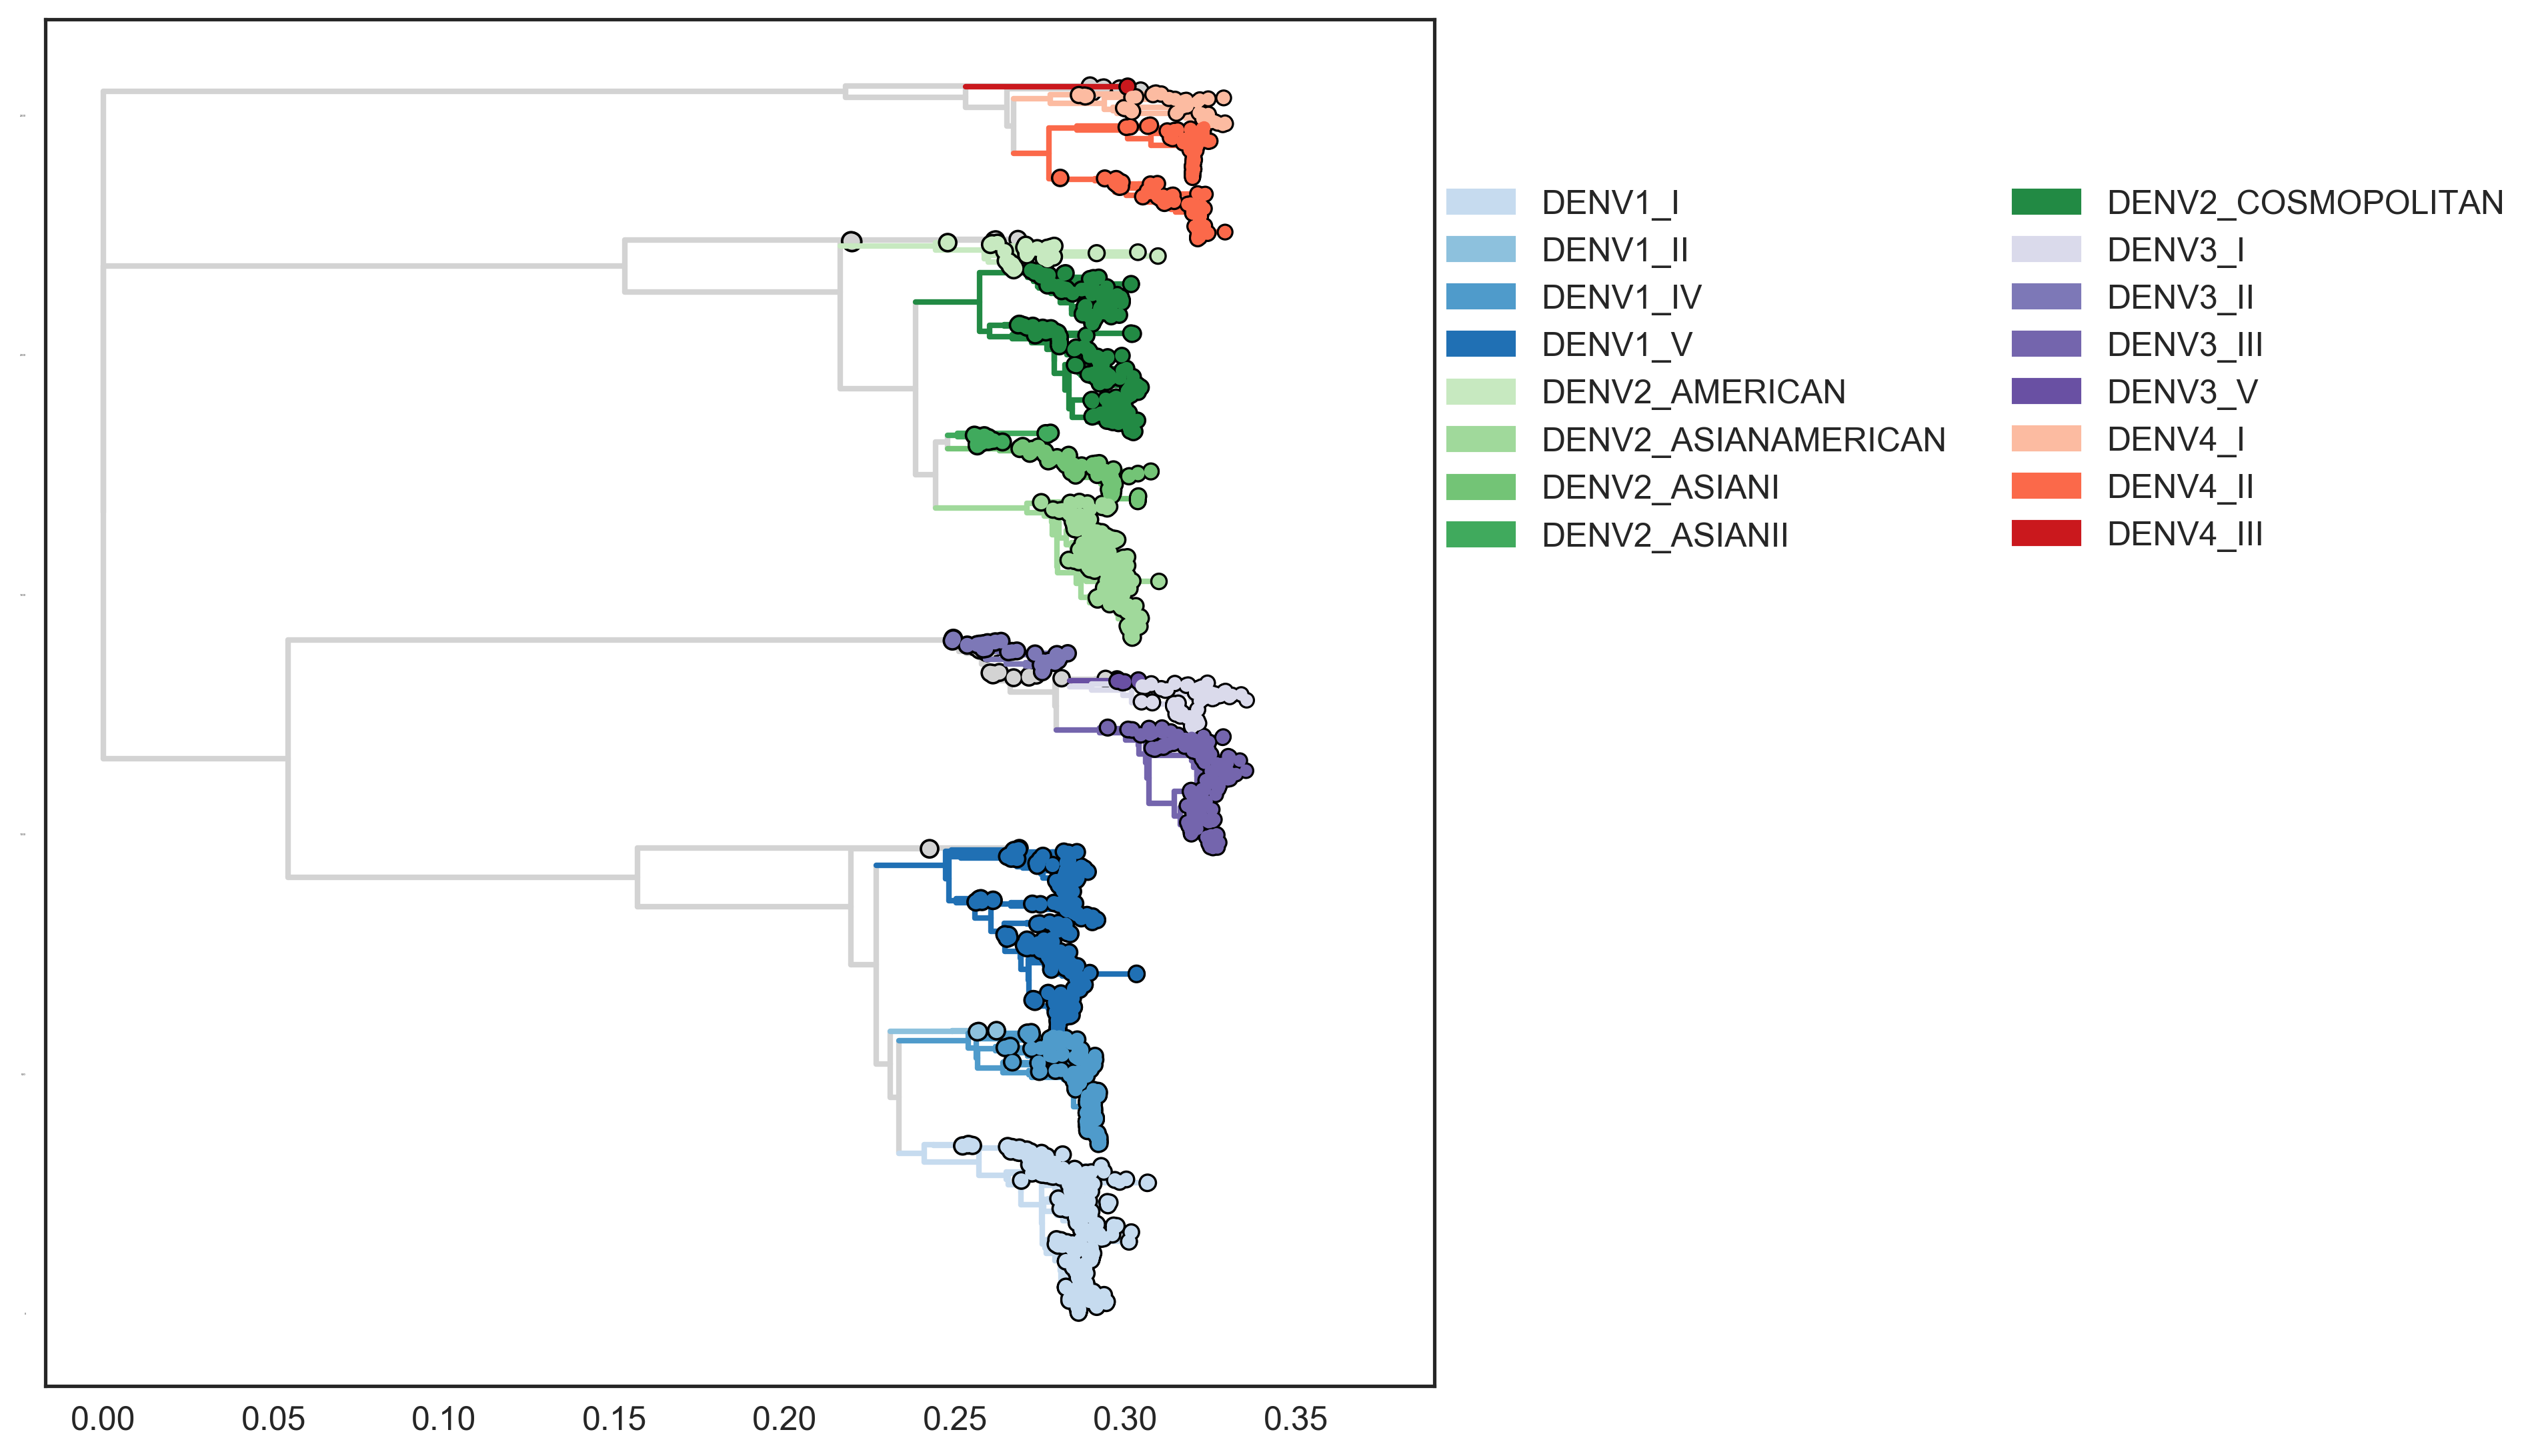
\includegraphics[width=\linewidth]{../figures/png/genotype_tree.png}
  	\caption{\textbf{Phylogeny of dengue viral sequences.}
    Maximum likelihood phylogeny of dengue virus genomes, colored by canonical genotype assignment.
    }
  	\label{genotype_tree}
  \end{centering}
\end{figure}

One explanation for these and similar observations (reviewed in *) is that overlooked intraserotype antigenic variation contributes to these genotype-specific case outcomes and epidemic patterns.
Recent efforts to antigenically characterize diverse DENV viruses suggests that each serotype may contain antigenic heterogeneity, but the source and impact of this heterogeneity is not clear*.
Here, we take a phylogenetic approach to characterize the evolutionary basis for observed antigenic heterogeneity among DENV clades.
We also quantify the impact of within- and between-serotype antigenic variation on real-world DENV population dynamics.

\section*{Results}

\subsection*{Dengue neutralization titer data}

Antigenic distance between a pair of viruses $i$ and $j$ is experimentally quantified using neutralization titer, which measures how well serum drawn after infection with virus $i$ is able to neutralize virus $j$ in vitro.
To measure the pairwise antigenic distances for a panel of diverse DENV viruses (Figure~\ref{titered_strains_tree}), Katzelnick et al*. infected naive non-human primates (NHP) with each virus, drew sera at three months post-infection, and then titered this sera against a panel of test viruses.
To compare patterns of cross-protection in NHP and humans, they also drew sera from 31 study participants six weeks after inoculation with a monovalent component of the NIH dengue vaccine candidate.
This sera was also titered against a broad panel of DENV viruses.
As reported by Katzelnick et al.*, we find generally consistent patterns of neutralization between the NHP and human sera data; see [ref*] for a detailed comparison.
In total, our dataset consists of 454 NHP sera titrations spanning the breadth of DENV diversity, and 728 human sera titrations providing deep coverage of a small subset of viruses.

To standardize these measurements, we first take the log$_2$ of each value, such that one titer unit corresponds to one, two-fold drop in neutralization.
We then define antigenic distance between autologous virus-sera pairs (i.e., virus $i$ and serum $i$) as zero.
Normalized antigenic distance between $i$ and $j$ are thus calculated as $D_{ij} = \mathrm{log}_2(T_{ii}) - \mathrm{log}_2(T_{ij})$, such that a higher value of $D_{ij}$ indicates that serum $i$ is less effective at neutralizing virus $j$, implying greater antigenic distance between viruses $i$ and $j$*.

The full dataset of standardized titer values is shown in Figure~\ref{titer_heatmap}.
Here, we see that homotypic virus-serum pairs are more closely related antigenically than heterotypic pairs.
However, we also observe large variance around this trend, both within and between serotypes.
This suggests that treating each serotype as antigenically uniform overlooks potentially important antigenic heterogeneity across viruses within each serotype.

\begin{figure}[h]
\begin{centering}
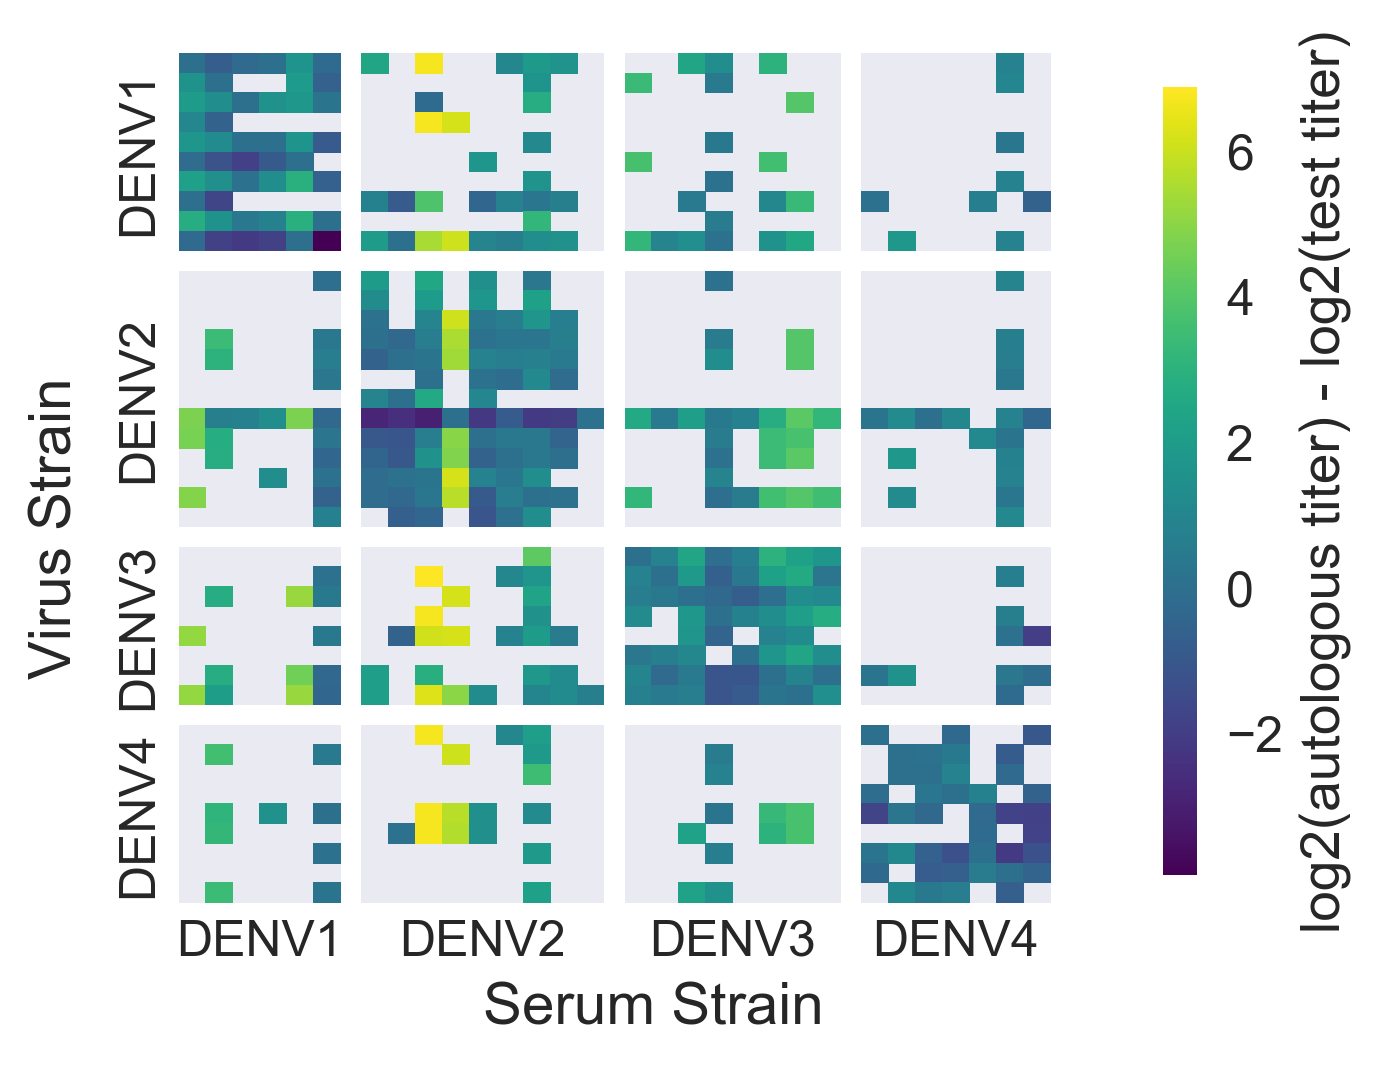
\includegraphics[width=0.65\textwidth]{../figures/png/titer_heatmap.png}
    \caption{\textbf{Normalized antigenic distance between pairs of dengue viruses and sera.}
    Aggregated neutralization titers from Katzelnick et al. are standardized such that the distance between autologous virus-serum pairs is 0, and each titer unit corresponds to one, two-fold change in PRNT50 value.
    Light gray areas represent missing data.
    Higher values correspond to greater antigenic distance.
    }
     \label{titer_heatmap}
\end{centering}
\end{figure}

\subsection*{Dengue antigenic evolution corresponds to phylogenetic divergence}

\begin{figure}[h]
  \begin{centering}
  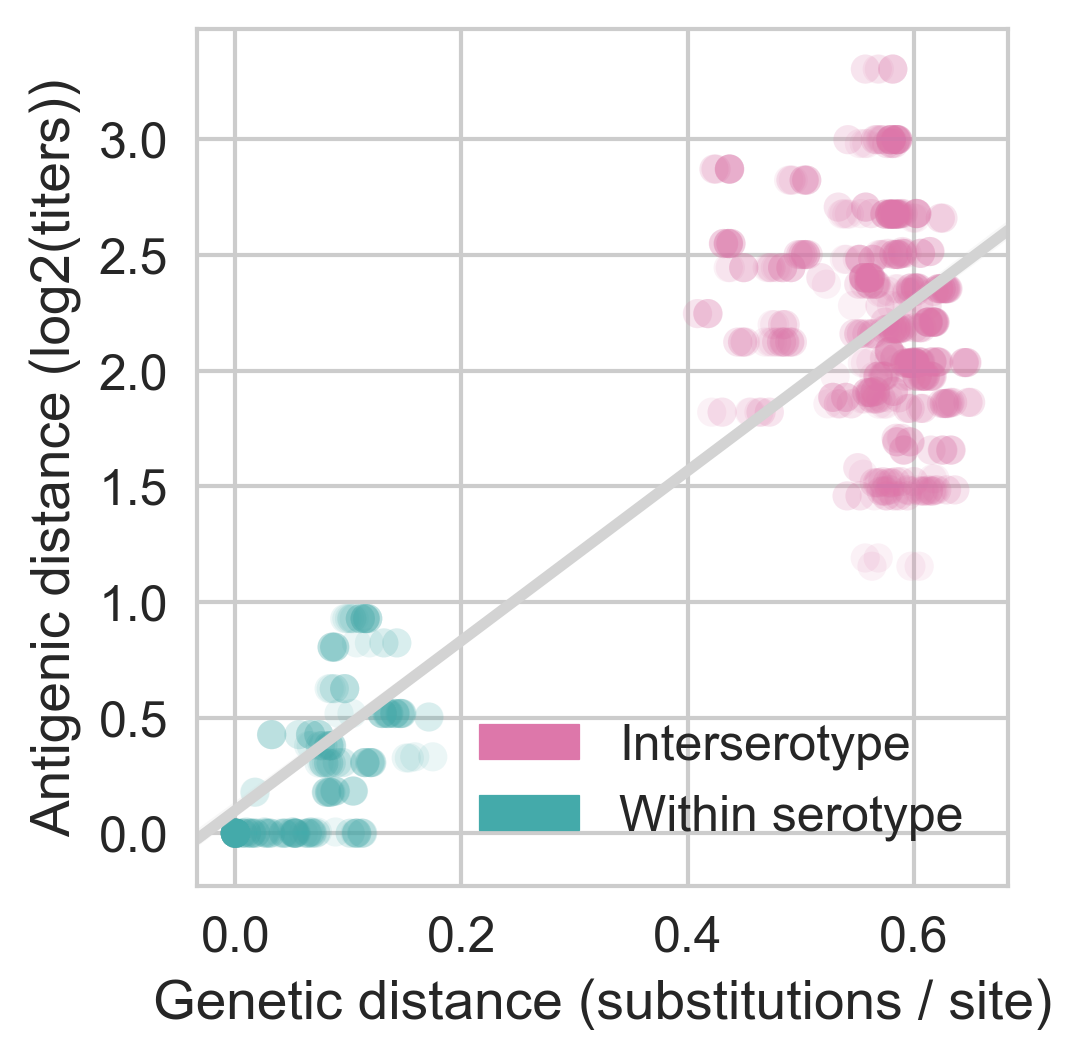
\includegraphics[width=0.6\textwidth]{../figures/png/genetic_antigenic_distance.png}
  	\caption{\textbf{Normalized antigenic distance vs. genetic distance between pairs of dengue viruses.}
    Antigenic distances are the same as from Figure~\ref{titer_heatmap};
    genetic distances are the patristic distances between viral genomes on a maximum likelihood phylogeny.
    }
  	\label{genetic_antigenic_distance}
  \end{centering}
\end{figure}

Titer measurements are prone to noise*, and there is a limited amount of available titer data.
If the antigenic heterogeneity observed in the raw data is truly the result of an underlying evolutionary process, we expect that changes in antigenic phenotype correspond to underlying changes in viral genotype.
Figure~\ref{genetic_antigenic_distance} shows the relationship between genetic and antigenic distance between each pair of viruses in our dataset.
There are two groups of comparisons --- between serotype and within serotype --- however, even within serotypes there is significant genetic diversity and a correlation between increased genetic distance and increased antigenic distance.
The relationship between genetic distance and antigenic distance is consistent within and between serotypes, where increasing genetic divergence generally corresponds to increased antigenic distance.

\subsection*{Antigenic evolution occurs within serotypes}
To fully map the relationship between DENV genetic and antigenic evolution, we adapt a phylogeny-based model originally developed for influenza*.
Conceptually, this model predicts titer values through three steps.
First, we build a phylogeny of dengue virus sequences to establish the genetic relationships between viruses (Figures~\ref{genotype_tree}, \ref{sequence_distribution}).
Next, we infer how much antigenic change has occurred along each branch of the phylogeny by mapping titer changes to individual branches.
This assigns each branch $b$ an antigenic distance $d_b$.
With this in hand, we estimate the antigenic distance between all pairs of viruses by tracing the path between them in the phylogeny, summing branch-specific distances $d_b$ as we go (Methods, Eq.~\ref{eq_predicted_titers}).

To learn these values of $d_b$, we first split our dataset into training (random 90\% of measurements) and test data (the remaining 10\% of values).
We take the training data and fit $d_b$ for each branch in the tree, subject to regularization as follows (also detailed in Methods, Eq.~\ref{eq_cost_fn}).
Parsimoniously, we expect that antigenic change is more likely to occur through larger changes on a few branches than through small changes on many branches; correspondingly, our prior expectation of values of $d_b$ is exponentially distributed such that most values of $d_b = 0$.
This is analogous to lasso regression to identify a few parameters with positive weights and set other parameters to 0.
Additionally, some viruses have greater binding avidity, and some sera are more potent than others (Figure~\ref{titer_asymmetry}); these `row' and `column' effects, respectively, are normally distributed and are taken into account when estimating titers.
The model uses convex optimization to learn the values of $d_b$ that minimize the sum of squared errors (SSE) between observed and predicted titers in the training data.

\begin{figure}[h]
  \begin{centering}
    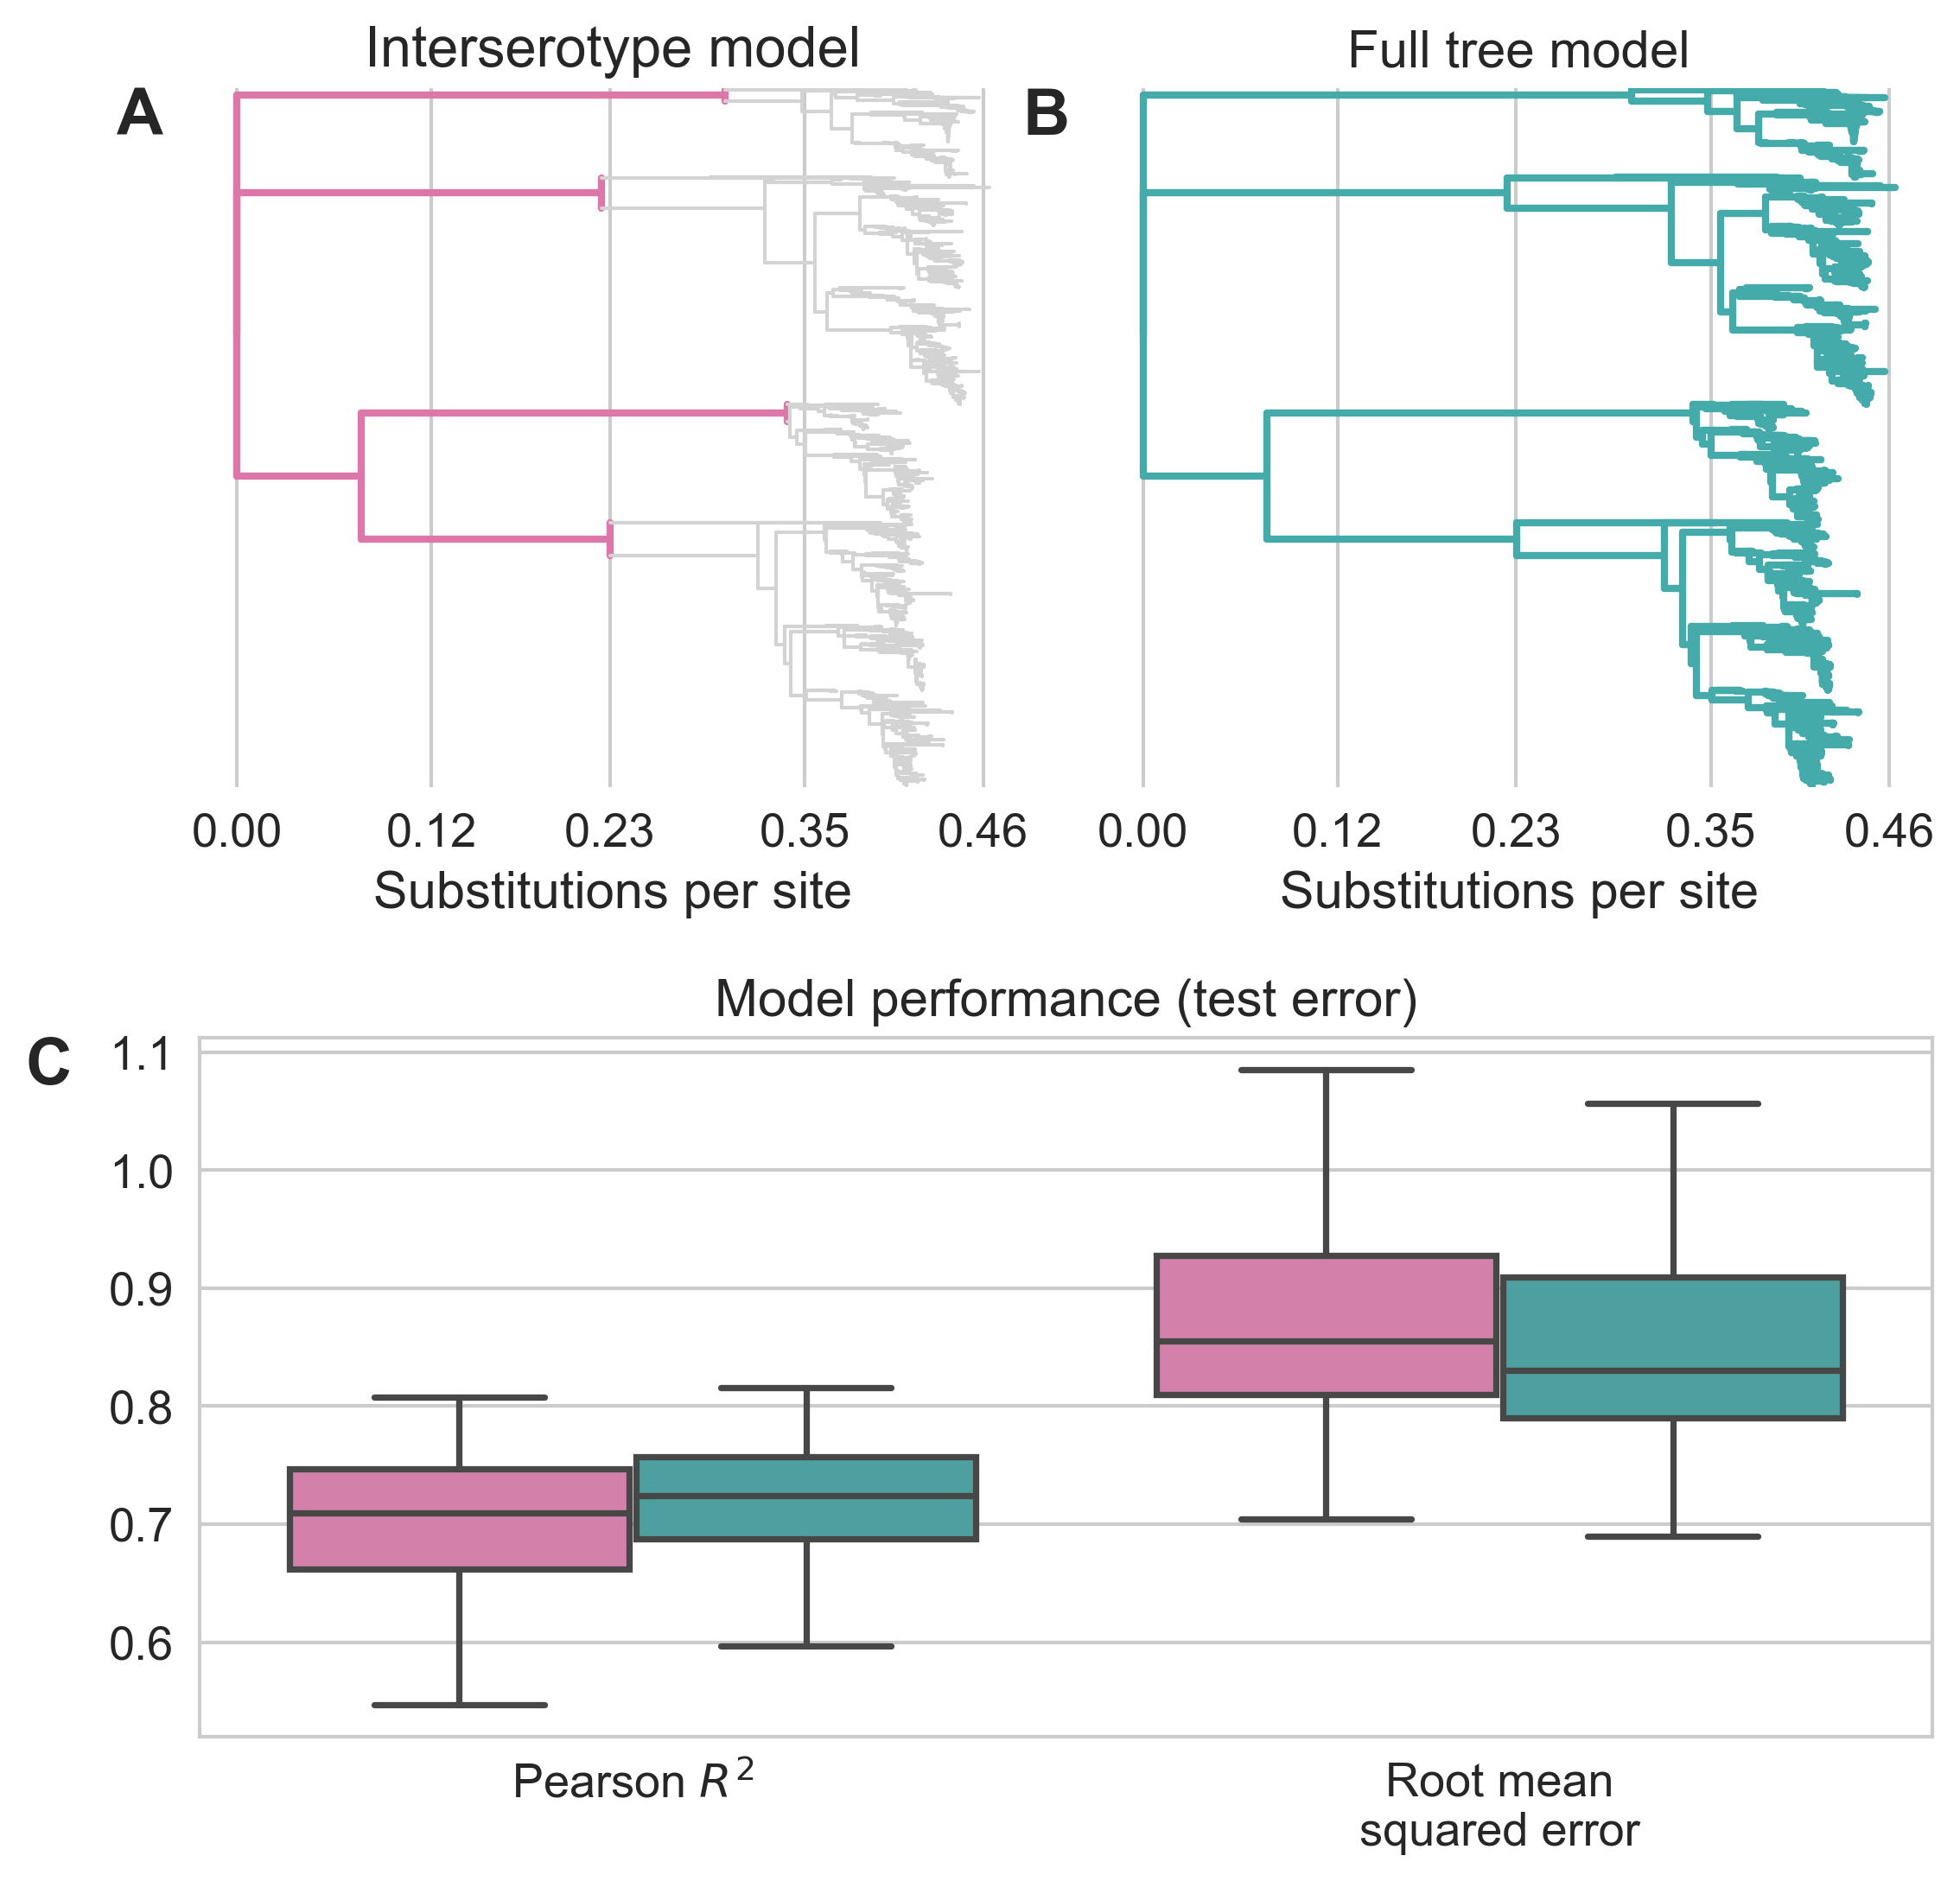
\includegraphics[width=0.8\textwidth]{../figures/png/titer_model_performance.png}
        \caption{\textbf{Titer model formulations and performance.}
        \textbf{A} The `interserotype model' only allows branches that lie between serotypes to contribute to antigenic evolution.
        All other branches are assigned $d_b = 0$.
        \textbf{B} The `full tree model' allows any branch in the phylogeny to contribute to antigenic evolution ($d_b >= 0$).
        \textbf{C,D} Predictive performance of each model on the test dataset (aggregated from 10-fold cross-validation).
        Shading represents the 95\% confidence interval.
        }
         \label{titer_model_performance}
  \end{centering}
\end{figure}

This model formulation is an effective tool for estimating antigenic relationships between viruses based on their relative positions in the phylogeny.
We can use variations of this model to explicitly test whether the observed antigenic phenotypes are better explained by the hypothesis that dengue serotypes are antigenically uniform (`interserotype model'), or by the hypothesis that serotypes are antigenically diverse (`full tree model').
In the interserotype model, we set $d_b = 0$ for all branches in the tree that do not lie between serotypes (Figure~\ref{titer_model_performance}A).
Alternatively, the `full tree model' allows any branch in the phylogeny to contribute to antigenic evolution (Figure~\ref{titer_model_performance}B).
For each model, we learn model parameters from the training data, and then use those parameters to predict test data values.
We assess model performance by comparing the predicted test titer values to the actual values.
Model performance indicates how well the hypothesis embedded in the model explains the observed data.

We find that serotype-level characterization alone explains observed antigenic phenotypes to a reasonable degree.
On average, this interserotype model predicts titers within 1.02 log$_2$ titer units of the true value (root mean squared error, RMSE), and explains 62\% of the observed variation in neutralization titers overall (Figure~\ref{titer_model_performance}).

However, we find that accounting for within-serotype antigenic evolution substantially improves our ability to explain dengue antigenic phenotypes.
The full tree model is able to predict test titers within 0.86 log$_2$ titer units of the true value (RMSE approaching the level of error intrinsic to the assay), and explains 74\% of the observed variation in neutralization titers overall (Figure~\ref{titer_model_performance}).
Importantly, all reported error metrics refer to performance on test data, so this difference in model performance is not due to the number of free parameters.
The full tree model performance is comparable to the model error from a cartography-based characterization of the same dataset* (RMSE 0.65--0.8 log$_2$ titer units), and to the error observed when this model was used to characterize an influenza dataset (RMSE of 0.5 log$_2$ titer units)*.
From this, we conclude that there is antigenic evolution within each serotype of DENV, and that this is driven by underlying genetic divergence.

Collapsing putatively antigenically uniform clades, we observe at least 12 distinct antigenic phenotypes of DENV (Figure~\ref{antigenic_tree}) and reject the null hypothesis that all DENV viruses within a serotype are antigenically uniform.
The titer dataset spans the breadth of canonical DENV genotypes, but in most cases lacks the resolution to detect within-genotype antigenic diversity.
We thus expect that these results represent a lower-bound on the true extent of DENV intraserotype antigenic diversity.

\begin{figure}[h]
  \begin{centering}
    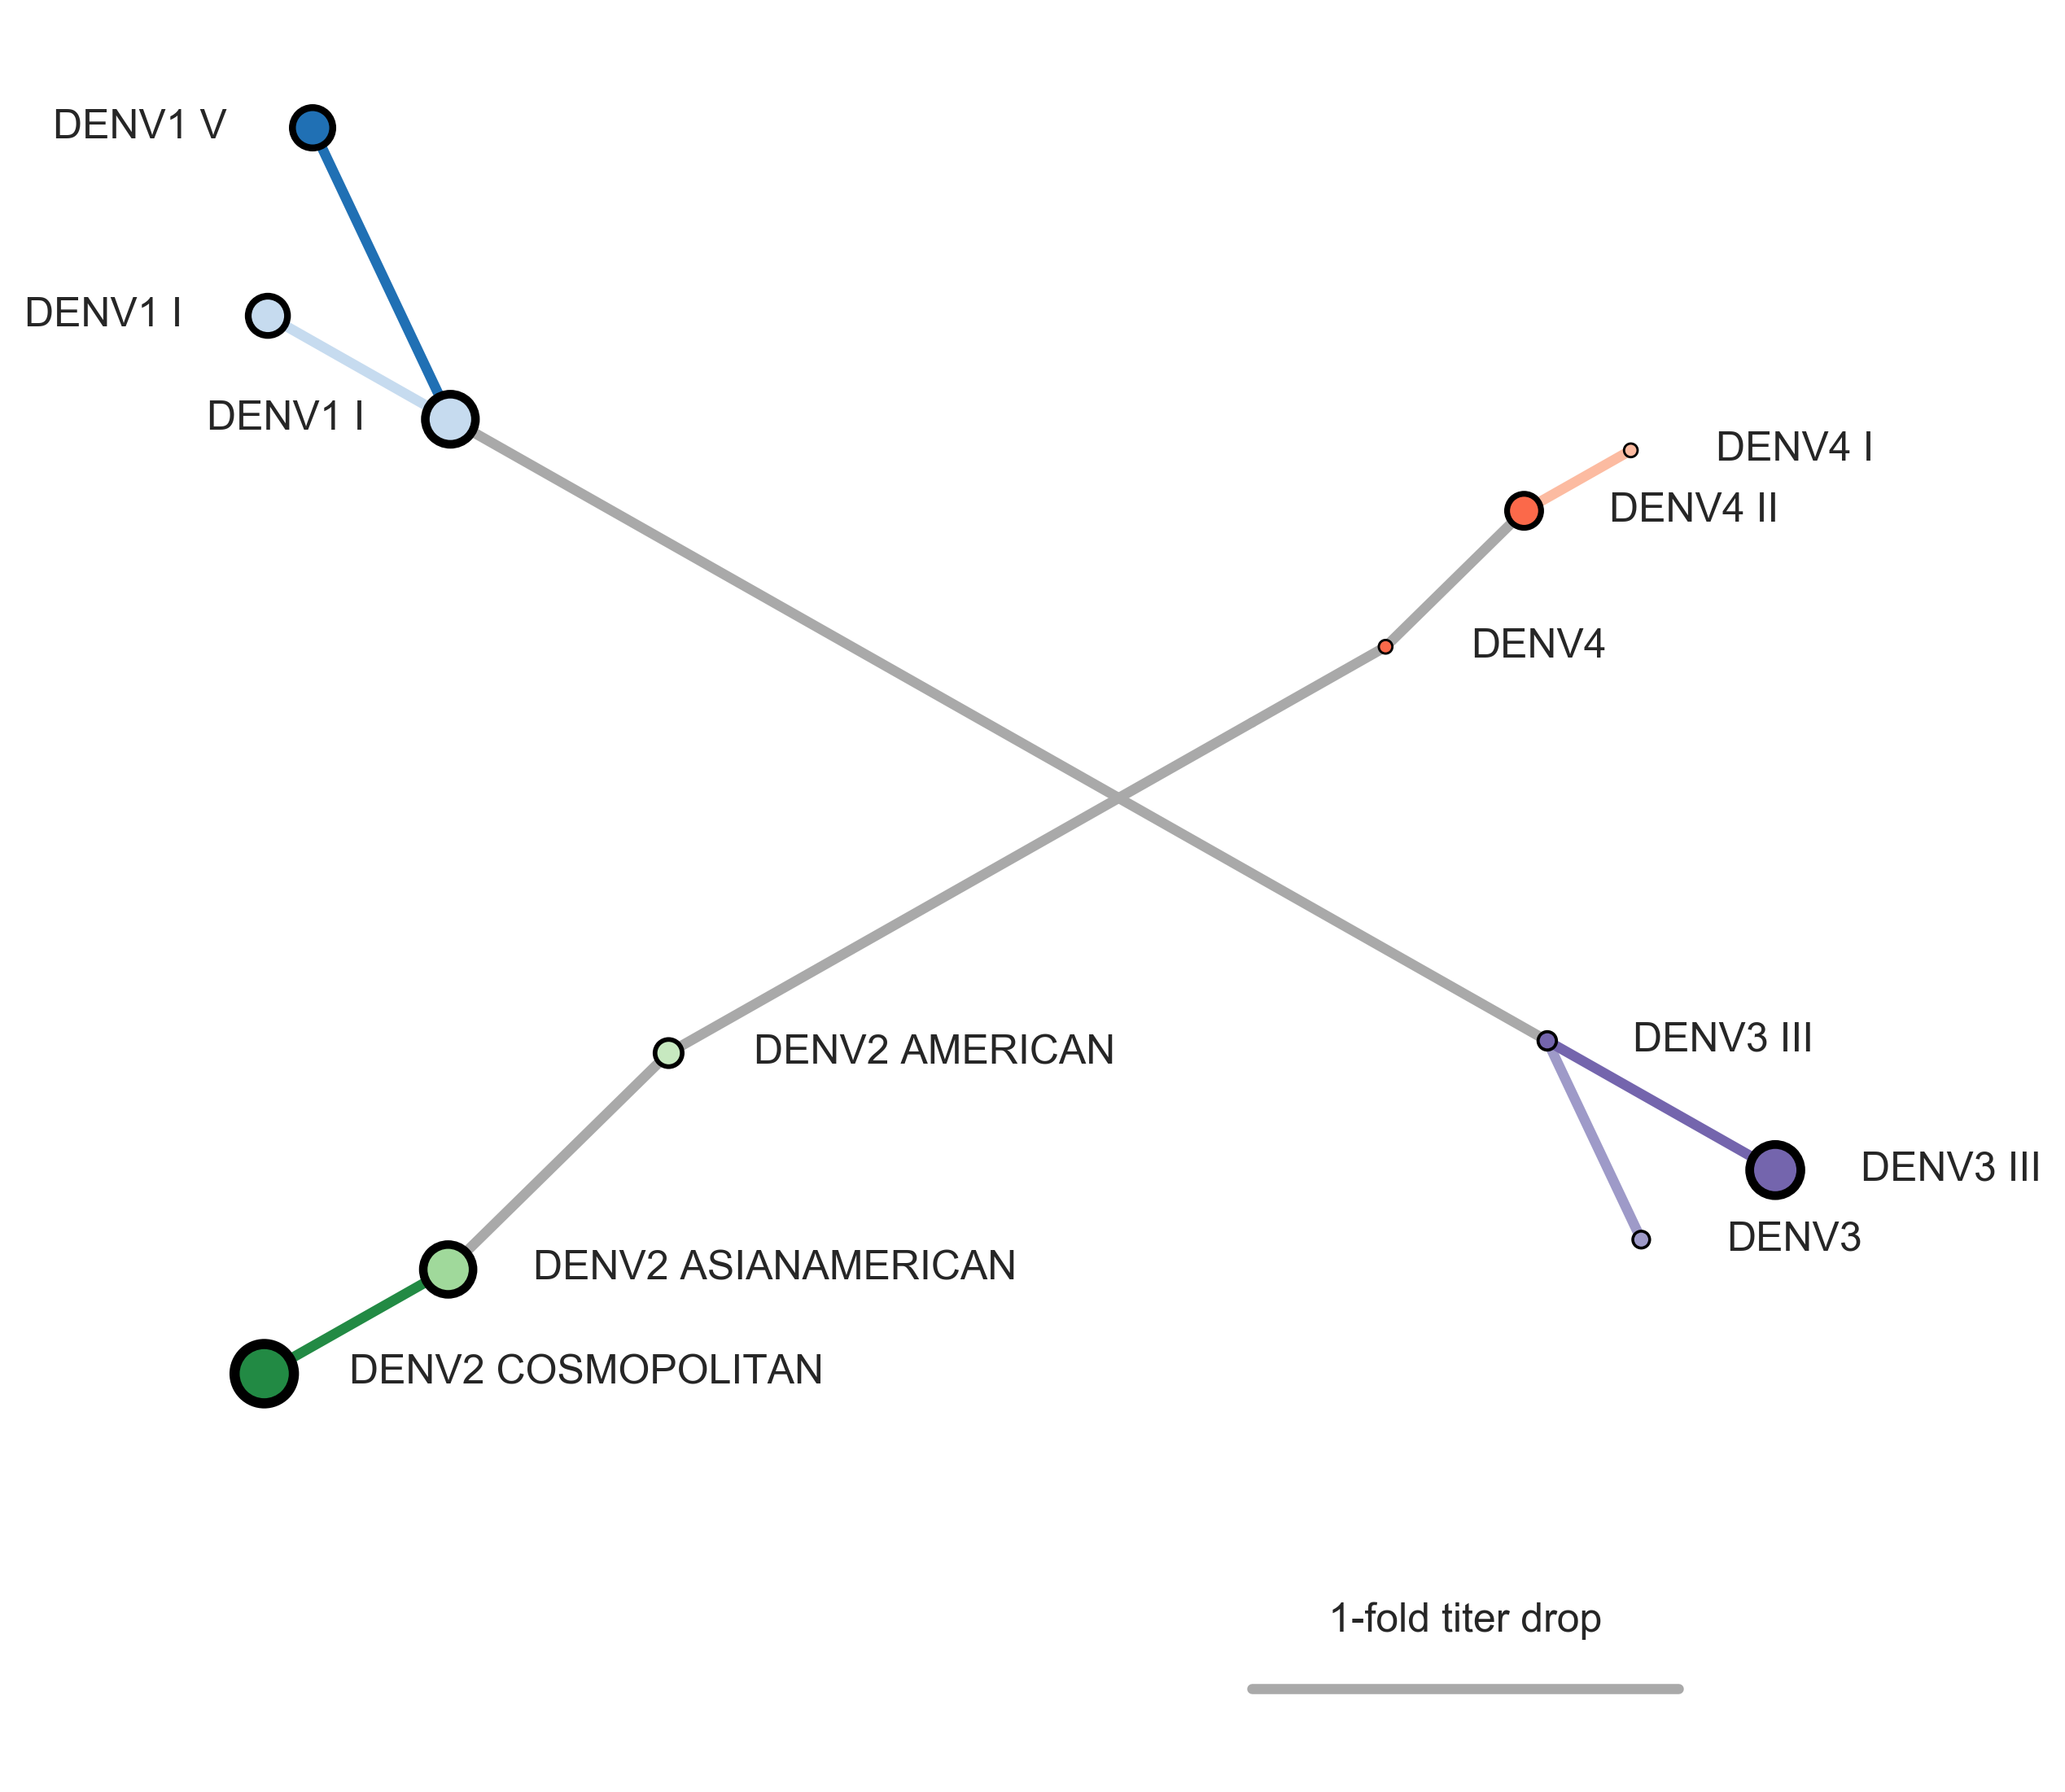
\includegraphics[width=\linewidth]{../figures/png/antigenic_tree.png}
    \caption{\textbf{Tree of dengue antigenic phenotypes.}
    We infer the topology from a maximum likelihood phylogeny of DENV genomes.
    Branch lengths are scaled to reflect $d_b$, the relative contributions of each branch to antigenic divergence, as inferred by the `full tree' model of DENV evolution.
    Antigenically uniform clades are collapsed, and node diameter reflects the size of the collapsed clade.
    Figure~\ref{antigenic_tree_supplement} offers an additional view of the same topology.
    }
     \label{antigenic_tree}
  \end{centering}
\end{figure}

\subsection*{Antigenic novelty predicts serotype success}
From the titer model, we observe strong evidence that homotypic genotypes of DENV vary in their ability to escape antibody neutralization (Figures~\ref{titer_model_performance}, \ref{genotype_dTiter_heatmap}).
However, antibody neutralization is only one of many factors that shape epidemic patterns.
We investigate whether the observed antigenic diversity influences dengue population dynamics in the real world.
The size of the viral population (i.e., prevalence, commonly analyzed using SIR models) is determined by many complex factors, and reliable values for population prevalence are largely unavailable.
Contrastingly, the composition of the viral population (i.e., the relative frequency of each viral clade currently circulating) can be estimated over time by examining historical sequence data*, and is primarily driven by viral fitness*.
In meaningfully antigenically diverse viral populations, antigenic novelty (relative to standing population immunity) contributes to viral fitness: as a given virus $i$ circulates in a population, the proportion of the population that is susceptible to infection with $i$--and other viruses antigenically similar to $i$--decreases over time as more people acquire immunity*.
Antigenically novel viruses that are able to escape this population immunity are better able to infect hosts and sustain transmission chains, making them fitter than the previously circulating viruses*.
Thus, if antigenic novelty constitutes a fitness advantage for DENV, then we would expect greater antigenic distance from recently circulating viruses to correlate with higher growth rates.

\begin{figure}[h]
  \begin{centering}
    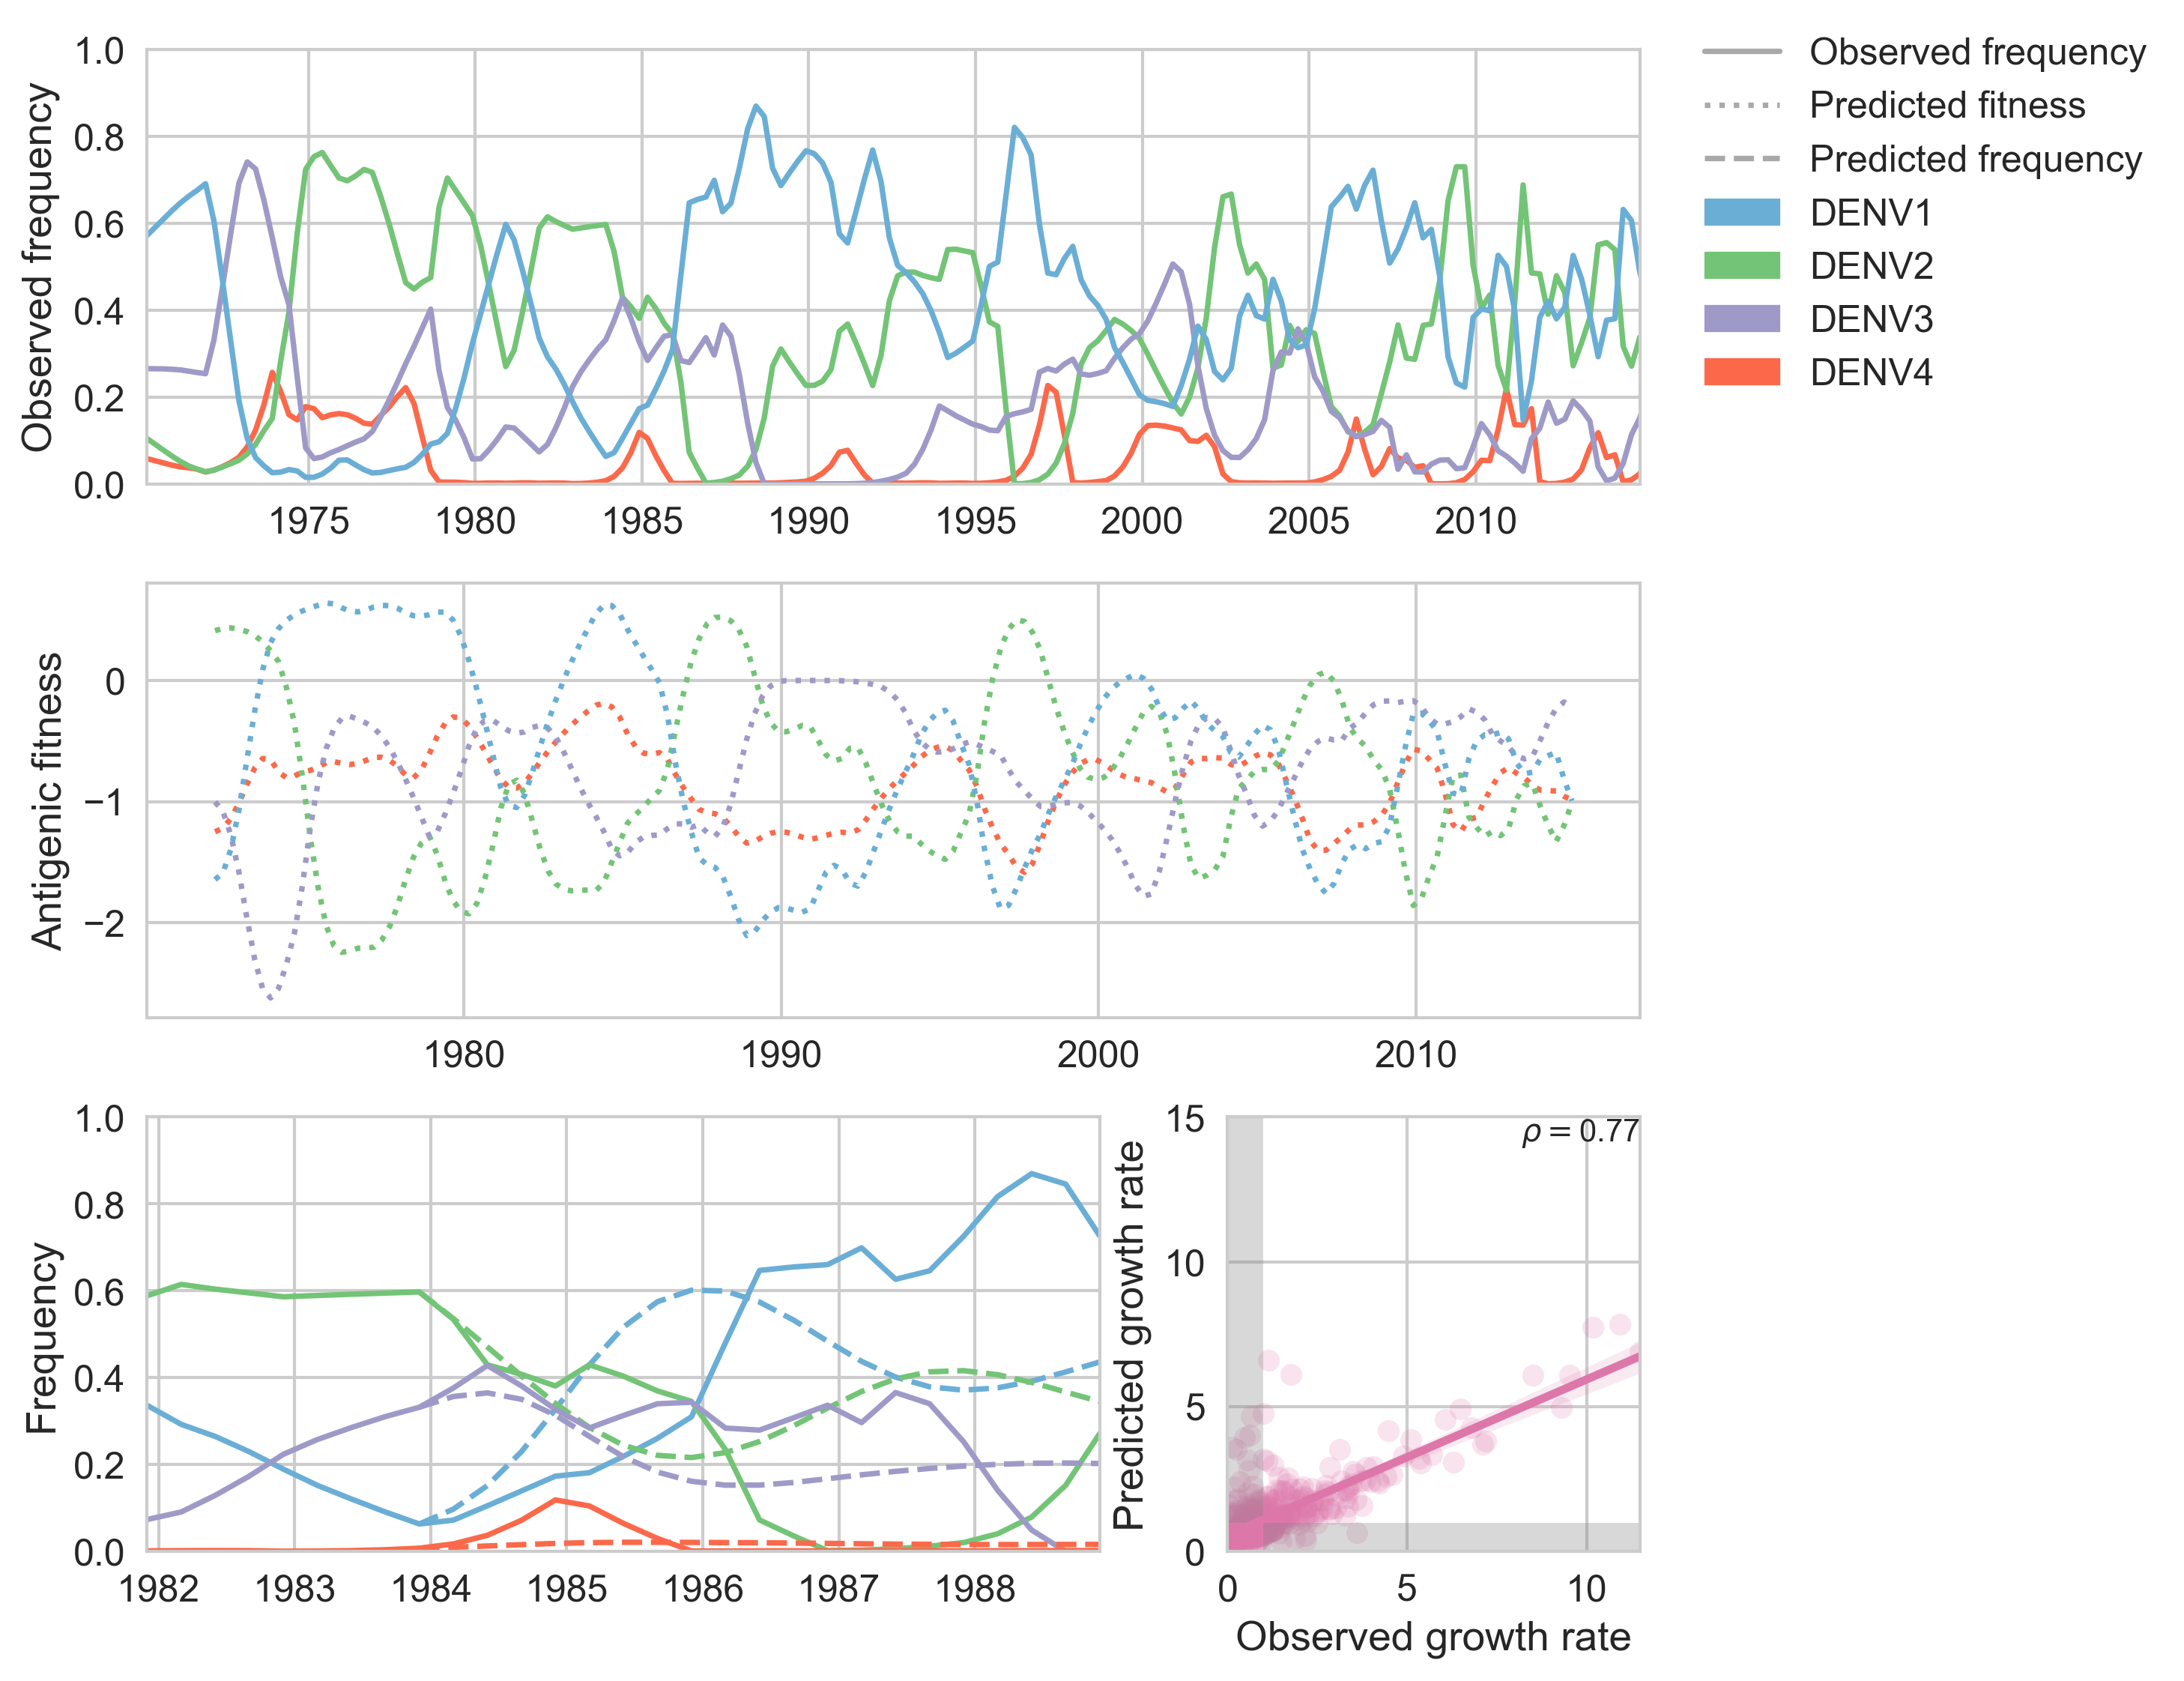
\includegraphics[width=\linewidth]{../figures/png/serotype_fitness_model.png}
  	\caption{\textbf{Antigenic novelty predicts serotype success.}
    \textbf{A} The relative frequency of each serotype, $x_i$, in Southeast Asia is estimated every three months based on available sequence data.
    \textbf{B} We calculate antigenic fitness for each serotype over time as its frequency-weighted antigenic distance from recently circulating viruses.
    \textbf{C} At each timepoint $t$, we blind the model to all empirical data from timepoints later than $t$ and predict each serotype's future trajectory based on its initial frequency, time-invariant intrinsic fitness, and antigenic fitness at time $t$ (Methods, Eq.~\ref{eq_predict_frequency}).
    We predict forward in three-month increments for a total prediction period of $dt = 5$ years.
    At each increment, we use the predicted stepwise frequency change to adjust our estimates of antigenic fitness on a rolling basis (Methods, Eq.~\ref{eq_compounding_immunity}).
    \textbf{D} Predicted growth rates are calculated as $\frac{\hat{x_i}(t+dt)}{x_i(t)}$ and compared to empirically observed growth rates.
    Serotype growth versus decline is accurate (i.e., the predicted and actual growth rates are both $>1$ or both $<1$, all points outside the gray area) for 80\% of predictions.
    }
  	\label{serotype_fitness_model}
  \end{centering}
\end{figure}

To test this hypothesis, we examine the composition of the dengue virus population in Southeast Asia from 1970 to 2015.
We estimate the relative population frequency of each DENV serotype at three month intervals, $x_i(t)$ (Figure~\ref{serotype_fitness_model}A), based on available sequence data (Methods, Eq.~\ref{eq_estimate_frequency}).

Fitter virus clades increase in frequency over time, such that $x_i(t+dt) > x_i(t)$.
It follows that these clades have a growth rate--defined as the fold-change in frequency over time--greater than one: $\frac{x_i(t+dt)}{x_i(t)} > 1$.
To isolate the extent to which antigenic fitness contributes to clade success and decline, we extend work by * to build a simple model that attempts to predict clade growth rates based on two variables: the antigenic fitness of the clade at time $t$, and a time-invariant free parameter representing the intrinsic fitness of the serotype the clade belongs to.
We estimate the antigenic fitness of clade $i$ at time $t$ as a function of its antigenic distance from each viral clade $j$ that has circulated in the same population over the previous two years, weighted by the relative frequency of $j$ and adjusted for waning population immunity (Figure~\ref{serotype_fitness_model}B; Methods, Eq.~\ref{eq_waning_immunity}).
Growth rates are estimated based on a five year sliding window (Figure~\ref{serotype_fitness_model}C).

This simple model explains 62\% of the observed variation in serotype growth rates, and predicts serotype growth vs decline correctly for 80\% of predictions (Figure~\ref{serotype_fitness_model}D).
This strongly suggests that antigenic fitness is a major driver of serotype population dynamics.
This also demonstrates that this model captures key components of dengue population dynamics; examining the formulation of this model in more detail can yield insights into how antigenic relationships influence DENV population composition.
The fitness model includes eight free parameters that are optimized such that the model most accurately reproduces the observed fluctuations in DENV population composition (reduction in prediction error relative to a null model, see Methods).
We find that serotype fluctuations are most consistent with a model wherein population immunity wanes linearly over time, with the probability of protection dropping by about 48\% per year for the first two years after primary infection.
We also find that these dynamics are best explained by intrinsic fitness that moderately varies by by serotype (Table~\ref{parameter_values}).

\subsection*{Antigenic novelty also partially predicts genotype success}
To estimate how well antigenic fitness predicts genotype dynamics, we used the same model to predict genotype success and decline.
As before, fitness of genotype $i$ is based on the intrinsic fitness of the serotype $i$ belongs to, and the antigenic distance between $i$ and each other genotype, $j$, that has recently circulated (Figure~\ref{genotype_fitness}B).
Importantly, we can calculate antigenic distance between $i$ and $j$ at the serotype level (i.e., the antigenic distances computed from the `interserotype model' as illustrated in Figure~\ref{titer_model_performance}A) or at the genotype level (i.e., the antigenic distances computed by the `full tree model' as illustrated in Figure~\ref{titer_model_performance}B, which incorporates the observed within-serotype heterogeneity).
If within-serotype antigenic heterogeneity contributes to genotype fitness, then we would expect estimates of antigenic fitness based on the `full tree model' to better predict genotype growth rates.

We find that antigenic fitness contributes to genotype turnover, although it explains less of the observed variation than for serotypes.
When antigenic distance is estimated from the `interserotype model', we find that our model of antigenic fitness explains approximately 31\% of the observed variation in genotype growth rates, and correctly predicts genotype growth vs. decline 68\% of the time (Figure~\ref{genotype_fitness}C).
Perhaps surprisingly, more precise estimates of antigenic distance between genotypes from the `full tree model' does not improve our predictions of genotype success ($R^2 = 0.28$, 70\% accuracy; Figure~\ref{genotype_fitness}D).
This suggests that although we find strong evidence that genotypes vary in their ability to escape neutralizing antibodies (Figures~\ref{titer_model_performance}, \ref{genotype_dTiter_heatmap}), these differences are subtle enough that they do not impact broad-scale regional dynamics over time.

\begin{figure}[h]
  \begin{centering}
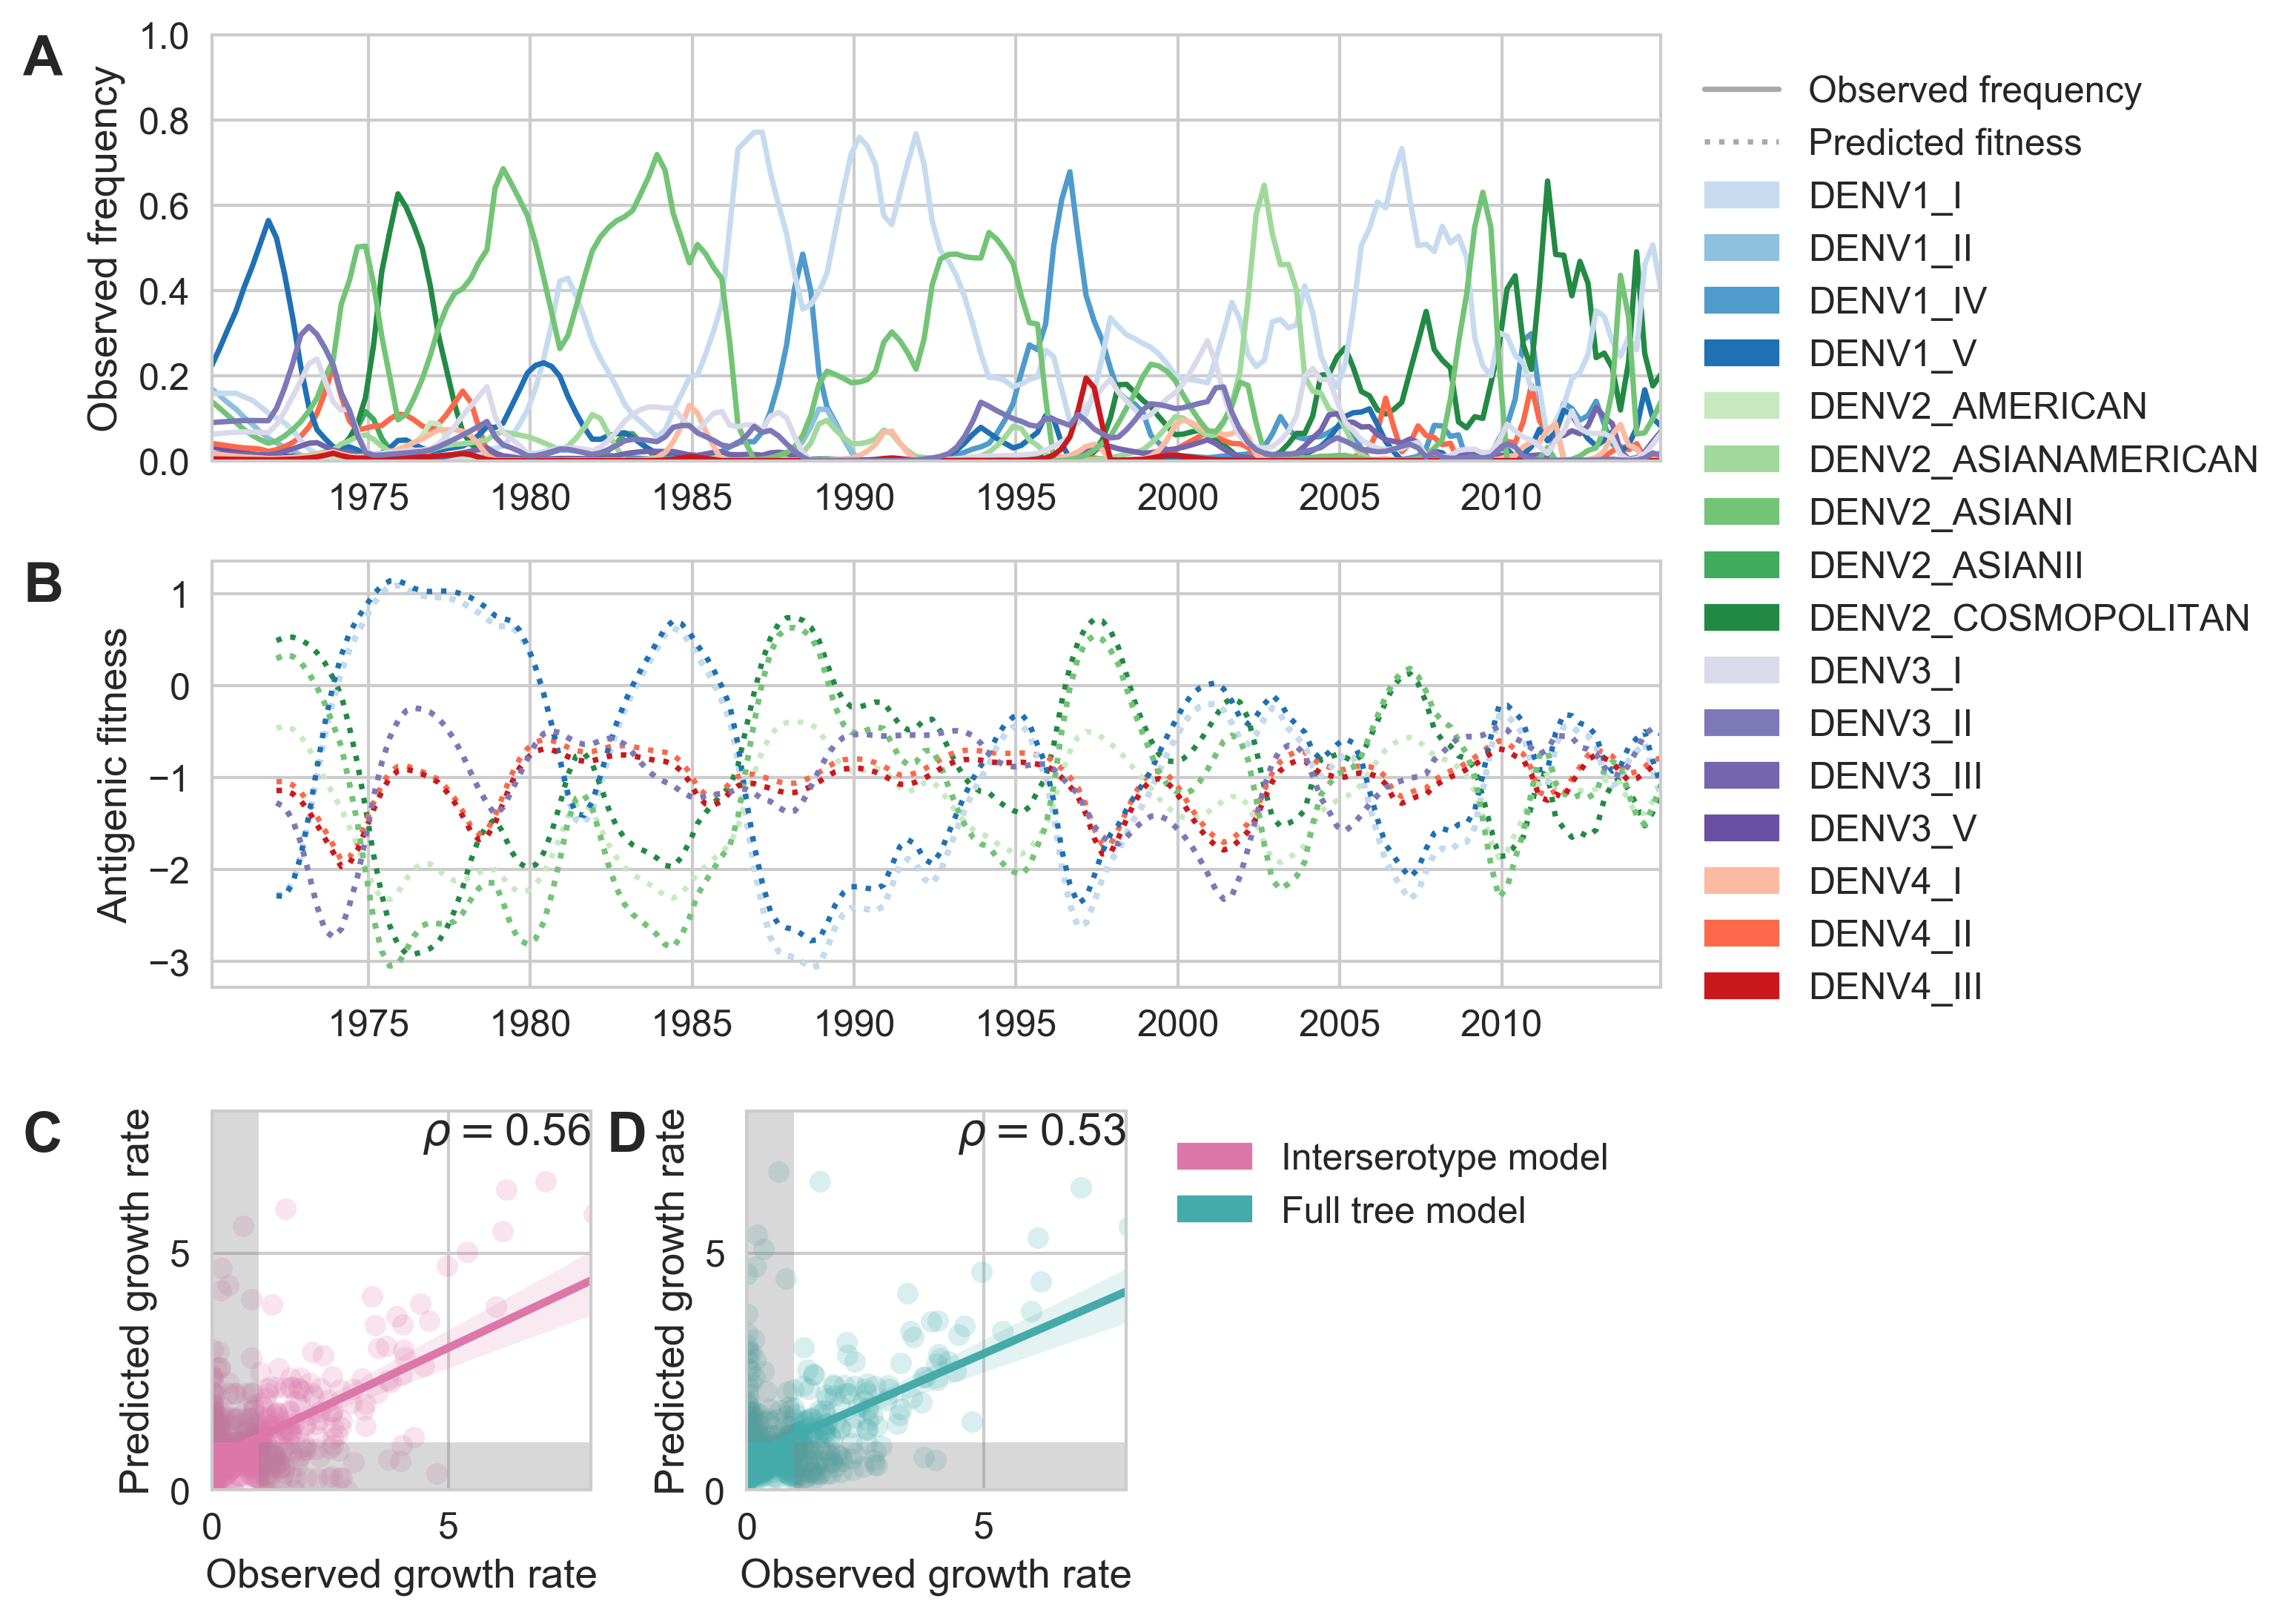
\includegraphics[width=\linewidth]{../figures/png/genotype-fitness.png}
    \caption{\textbf{Relative frequencies and fitness of dengue genotypes, 1970-2015.}
    \textbf{A} Relative frequencies of each canonical dengue genotype across Southeast Asia, estimated from available sequence data.
    \textbf{B} Antigenic fitness is calculated for each genotype as its frequency-weighted antigenic distance from recently circulating genotypes.
    We assess antigenic distance using either the `full tree model' or the `interserotype model' of antigenic relationships (Figure~\ref{titer_model_performance}).
    In this panel, we show antigenic fitness over time as derived from the `full tree model' estimates of antigenic distance.
    \textbf{C, D}  Fitness estimates were used to predict clade growth rates over 5 years, compounding immunity every three months based on predicted frequency changes (Methods Eq.~\ref{eq_compounding_immunity}).
    Here, we compare observed vs predicted growth rates for both formulations of the fitness model (using fitness derived from either the `interserotype' or `full tree' model estimates of antigenic distance).
    Growth versus decline was accurate (predicted and actual growth rates both $> 1$ or both $< 1$, points outside the gray shaded area) for 68\% -- 70\% of predictions, respectively.
}
     \label{genotype_fitness}
   \end{centering}
\end{figure}

\pagebreak

\section*{Discussion}

\subsection*{Within-serotype antigenic heterogeneity}
We show that mapping antigenic change to individual branches and interpolating across the DENV phylogeny is able to explain a large majority of the observed variation in antigenic phenotypes, as measured by neutralization titers.
This demonstrates that DENV antigenic divergence is closely coupled to genetic divergence.
We also find that accounting for within-serotype antigenic evolution is necessary to explain the observed variation in antigenic phenotypes.
This supports and expands upon previous reports* that the null hypothesis of antigenically uniform serotypes is inconsistent with observed patterns of cross-protection and susceptibility.
We observe at least 12 distinct antigenic phenotypes that are both genetically and antigenically distinct.
Analysis of the recent CYD-TDV vaccine trial shows different vaccine efficacy against genotypes I and II of DENV4*; the antigenic distance between these two genotypes is comparable to the antigenic distance separating each of the 12 antigenic phenotypes we report (Figures~\ref{antigenic_tree}, \ref{genotype_dTiter_heatmap}).
This suggests that these phenotypes may be sufficiently distinct to have important impacts on secondary case outcomes and vaccine efficacy.

Overall, we expect that these antigenic phenotypes represent a lower-bound on the extent, magnitude, and nature of antigenic heterogeneity with DENV.
Our current titer dataset spans the breadth of DENV diversity, but due to small sample size, it lacks the resolution to detect most sub-genotype antigenic variation or to identify which specific mutations correspond to changes in antigenic phenotype.
The appearance of the deep antigenic divergence of the four serotypes, and the more recent antigenic divergences within each serotype, suggest that DENV antigenic evolution is likely an ongoing, though gradual, process.
We therefore expect that future studies with richer datasets will find additional antigenic variation within each genotype.
This dataset also contains many left-censored titer values, where we know two viruses are at least $T$ titer units apart, but do not know exactly how far apart.
If we knew the true value of these censored titers, many of them would indicate larger antigenic distances than the reported values, $T$, which are used to train the model.
Thus, it is likely that our model systematically underestimates the magnitude of titer distances.
Finally, antibody neutralization and escape (as measured by PRNT titers) is only one component of the immune response to DENV.
Although analysis of a longitudinal cohort study shows that these neutralization titers correlate with protection from severe secondary infection*, it is unclear how PRNT titers correspond to antibody-dependent enhancement.
It is also important to note that DENV case outcomes are partially mediated by interactions with innate and T-cell immunity, the effects of which are not captured in neutralization titers*.
Overall, while richer datasets and the development of more holistic assays will be required in order to fully characterize the extent of DENV antigenic diversity, it is clear that the four-serotype model is insufficient to explain DENV antigenic evolution.

\subsection*{Viral clade dynamics}
We use these inferred antigenic relationships to directly quantify the impact of antigenic fitness on DENV population composition.
To do so, we measure serotype frequencies across Southeast Asia over time and construct a model to estimate how they will fluctuate (Methods, Eq.~\ref{eq_population_immunity}--\ref{eq_delta_sse}).
This model places a fitness value on each serotype that derives from a constant intrinsic component alongside a time-dependent antigenic component.
Antigenic fitness declines with population immunity, which is accumulated via the recent circulation of antigenically similar viruses.
We find that antigenic fitness is able to explain most of the observed variation in serotype growth and decline (Figure~\ref{serotype_fitness_model}).
This demonstrates that antigenic fitness is a strong determinant of DENV serotype dynamics in a real-world, hyperendemic population.

We similarly use this model to quantify the effect of within-serotype antigenic variation on the success and decline of canonical DENV genotypes (Figure~\ref{genotype_fitness}).
As above, genotype antigenic fitness declines with population immunity.
Here, we estimate population immunity based on antigenic distance from recently circulating genotypes, using distances derived from the `interserotype model' or the `full tree model' of DENV antigenic evolution.
We then directly compare how strongly these coarser serotype-level versus specific genotype-level antigenic relationships impact DENV population dynamics.
Overall, we find that antigenic fitness explains a moderate portion of the observed variation in genotype growth and decline.
Surprisingly, however, we find that incorporating within-serotype antigenic differences does not improve our predictions (Figure~\ref{genotype_fitness}C,D).
This suggests that although genotypes are antigenically diverse, these differences do not appear to influence large-scale regional dynamics over time.

However, this observation is subject to caveats imposed by the the available data and model assumptions.
We estimate DENV population composition over time based on available sequence data, pooled across all of Southeast Asia (Methods, Eq.~\ref{eq_estimate_frequency}).
As the vast majority of cases of DENV are asymptomatic*, sequenced viruses likely represent a biased sample of more severe cases from urban centers where patients are more likely to seek and access care.
We also assume that Southeast Asia represents a closed viral population with homogeneous mixing.
However, increasing globalization likely results in some amount of viral importation that is not accounted for in this model.
Finally, although Southeast Asia experiences hyperendemic DENV circulation, the majority of DENV transmissions are hyper-local*, and viral populations across this broad region may not mix homogeneously each season.
Thus, it is possible that these sub-serotype antigenic differences impact finer-scale population dynamics, but we lack the requisite data to examine this hypothesis.

\subsection*{Conclusions}
We find that within-serotype antigenic evolution is necessary to explain the observed patterns of cross-immunity and susceptibility after primary DENV infection.
These within-serotype differences are large enough that we believe they likely impact secondary case outcomes and small scale population dynamics.
We also find that population immunity is a strong determinant of the composition of the DENV population across Southeast Asia, although this is putatively driven by coarser, serotype-level antigenic differences.
As richer datasets become available, future studies that similarly combine viral genomics, functional antigenic characterization, and population modeling have great potential to improve our understanding of how DENV evolves antigenically and moves through populations.

\subsection*{Model sharing and extensions}
We have provided all code, configuration files and datasets at `github.com/blab/dengue-antigenic-dynamics', and wholeheartedly encourage other groups to adapt and extend this framework for further investigation of DENV antigenic evolution and population dynamics.


\newpage

\section*{Methods}
\subsection*{Data}
\textbf{Sequences}\\
We downloaded all dengue virus sequences available from the Los Alamos National Lab Hemorrhagic Fever Virus Database* as of March 7, 2018, that contained the full coding sequence of E (total N=12,645).
We discarded sequences which were putative recombinants, duplicates, lab strains, or which lacked an annotated sampling location and/or sampling date.
We then randomly subsampled up to 8 viruses per region, per month, preferentially including records with available titer data and longer sequences.
Our final dataset consists of 2,563 viral sequences (Figure~\ref{sequence_distribution})

\textbf{Titers}\\

Antigenic distance between pairs of viruses $i$ and $j$ is experimentally measured using a neutralization titer, which measures how well serum drawn after infection with virus $i$ is able to neutralize virus $j$ in vitro*.
Briefly, two-fold serial dilutions of serum $i$ are incubated with a fixed concentration of virus $j$.
Titers represent the lowest serum concentration able to neutralize $50\%$ of virus, and are reported as the inverse dilution.
We used two publicly available plaque reduction neutralization titer (PRNT50) datasets generated by Katzelnick et al. in *.
The primary dataset was generated by infecting each of 36 non-human primates with a unique strain of DENV.
NHP sera was drawn after 12 weeks and titered against the panel of DENV viruses.
The secondary dataset was generated by vaccinating 31 human trial participants with a monovalent component of the NIH DENV vaccine.
Sera was drawn after 6 weeks and titered against the same panel of DENV viruses.
As discussed in Katzelnick et al.*, these two datasets show similar patterns of antigenic relationships between DENV viruses.
In total, our dataset includes 47 virus strains, 36 serum strains, and 1182 measurements.

\subsection*{Titer Model}
We compute standardized antigenic distance between virus $i$ and serum $j$ (denoted $D_{ij}$) from measured titers relative to autologous titers (denoted $T_{ii}$ and $T_{ij}$, respectively), such that
\begin{equation}
  \label{eq_titer_norm}
D_{ij} = \mathrm{log}_2(T_{ii}) - \mathrm{log}_2(T_{ij})
\end{equation}
To predict unmeasured titers, we employ the `tree model' from Neher et al.* and implemented in Nextstrain*, which assumes that antigenic evolution is driven by underlying genetic evolution.
Observed titer drops are mapped to branches in the viral phylogeny after correcting for overall virus avidity, $v_i$, and serum potency, $p_j$ (`row' and `column' effects, respectively):
\begin{equation}
  \label{eq_predicted_titers}
\hat{D}_{ij} \approx D_{ij} = \sum_{b \in path(i,j)} d_b + v_i + p_j
\end{equation}
where $d_b$ is the titer drop assigned to each branch, $b$, in the phylogeny.
We randomly withhold 10\% of titer measurements as a test set.
We use the remaining 90\% of titer measurements as a training set to learn values for virus avidity, serum potency, and branch effects.
As in Neher et al.*, we formulate this as a convex optimization problem and solve for these parameter values to minimize the cost function:
\begin{equation}
  \label{eq_cost_fn}
C = \sum_{i,j} (\hat{D}_{ij} - D_{ij})^2 + \lambda \sum_{b} d_b + \gamma \sum_{i} v_i^2 + \delta \sum_{j} p_j^2
\end{equation}
Respectively, these terms represent the squared training error; an L1 regularization term on branch effects, such that most values of $d_b = 0$; and L2 regularization terms on virus avidities and serum potencies, such that they are normally distributed.
These parameter values are then used to predict the antigenic distance between all pairs of viruses, $i$ and $j$, in the phylogeny.
We assess performance by comparing predicted to known titer values in our test data set, and present test error (aggregated from 10-fold cross-validation) throughout the manuscript.

\subsection*{Viral Clade Dynamics}

\textbf{Empirical Clade Frequencies}\\
As discussed in Neher et al* and Lee et al*, we estimate empirical clade frequencies from 1970 to present based on observed relative abundance of each clade in the `slice' of the phylogeny corresponding to each quarterly timepoint.

Briefly, the frequency trajectory of each clade in the phylogeny is modeled according to a Brownian motion diffusion process discretized to three-month intervals.
Relative to a simple Brownian motion, the expectation includes an `inertia' term that adds velocity to the diffusion and the variance includes a term $x(1-x)$ to scale variance according to frequency following a Wright-Fisher population genetic process.
This results in the following diffusion process:
\begin{equation}
  \label{eq_estimate_frequency}
x(t+dt) = \mathcal{N}\left(x(t) + \epsilon dx, \; dt \sigma^2 x(t) (1-x(t))\right)
\end{equation}

with `volatility' parameter $\sigma^2$.
The term $dx$ is the increment in the previous timestep, so that $dx = x(t) - x(t-dt)$.
We used $\epsilon = 0.7$ and $\sigma = 2.0$ to maximize fit to empirical trajectory behavior.

We also include an Bernoulli observation model for clade presence / absence among sampled viruses at timestep $t$.
This observation model follows
\begin{equation}
f(x,t) = \Pi_{v \in V} x(t) \; \Pi_{v \notin V} (1-x(t))
\end{equation}
where $v \in V$ represents the set of viruses that belong to the clade and $v \notin V$ represents the set of viruses that do not belong to the clade.
Each frequency trajectory is estimated by simultaneously maximizing the likelihood of the process model and the likelihood of the observation model via adjusting frequency trajectory $\vec{x} = (x_1, ... x_n)$.

\textbf{Population Immunity}\\
For antigenically diverse pathogens, antigenic novelty represents a fitness advantage.
This means that viruses that are antigenically distinct from previously-circulating viruses are able to access more susceptible hosts, allowing the antigenically novel lineage to expand.
We adapt a simple deterministic model from {\L}uksza and L\"assig* to directly quantify dengue antigenic novelty and its impact on viral fitness.
We quantify population immunity to virus $i$ at time $t$, $P_i(t)$, as a function of which clades have recently circulated in the past $N$ years, and how antigenically similar each of these clades is to virus $i$:
\begin{equation}
  \label{eq_population_immunity}
P_i(t) = \sum_{n=1}^{n=N} \left(w(n)  \sum_{j} \Big( x_j(t-n) \, C( D_{ij}) \Big) \right)
\end{equation}
Where $D_{ij}$ is the antigenic distance between $i$ and each non-overlapping clade $j$, $n$ is the number of years since exposure, and $x_j(t-n)$ is the relative frequency of $j$ at year $t-n$.
Waning immunity is modeled as a non-negative linear function of time:
\begin{equation}
\label{eq_waning_immunity}
  w(n) = max(-\gamma n + 1, 0)
\end{equation}
The relationship between antigenic distance and the probability of protection, $C$, is also assumed to be linear and non-negative, such that:
\begin{equation}
C(D_{ij}) = max(-\sigma D_{ij} + 1, 0)
\end{equation}

We model the effects of population immunity, $P_i(t)$, on viral antigenic fitness, $f_i(t)$, as:
\begin{equation}
  \label{eq_fitness}
f_i(t) = f_0-\beta P_i(t)
\end{equation}
where $\beta$ and $f_0$ are fit parameters representing the slope of the linear relationship between immunity and fitness, and the intrinsic relative fitness of each serotype, respectively.

\textbf{Frequency Predictions}\\
Similar to the model implemented in {\L}uksza and L\"assig*, we estimate predicted clade frequencies at time $t + dt$ as
\begin{equation}
  \label{eq_predict_frequency}
\hat{x_i}(t+dt) = \frac{x_i(t) e^{f_i(t) dt}}{\sum_{i}x_i(t) e^{f_i(t) dt}}
\end{equation}
for short-term predictions (where $dt < 1$ year).

For long-term predictions, we must account for immunity accrued at each intermediate timepoint between $t$ and $dt$.
We divide the interval between $t$ and $dt$ into a total of $U$ 3 month timepoints, $[t+u, t+2u, ... t+U]$, such that $t+U=dt$.
We then compound immunity based on predicted clade frequencies at each intermediate timepoint:
\begin{equation}
\hat{x_i}(t+u) = x_i(t)e^{f_i(t) u}
\end{equation}
\begin{equation}
\hat{x_i}(t+2u) = \hat{x_i}(t+u) e^{f_i(t+u)u}
\end{equation}
$$...$$
\begin{equation}
\hat{x_i}(t+U) = x_i(t) e^{f_i(t)u} e^{f_i(t+u)u} e^{f_i(t+2u)u} ... e^{f_i(t+U)u}
\end{equation}
\begin{equation}
  \label{eq_compounding_immunity}
\hat{x_i}(t+dt) = \hat{x_i}(t+U) = x_i(t) e^{\sum_{u}f_i(t+u)u}
\end{equation}

We then calculate clade growth rates, defined as the fold-change in relative clade frequency between time $t$ and time $t+dt$:
\begin{equation}
  \label{eq_growth_rate}
\frac{\hat{x_i}(t+dt)}{x_i(t)}
\end{equation}

\textbf{Null model and model performance}\\
To quantify the impact of antigenic fitness on DENV clade success, we compare our antigenically-informed model to a null model wherein all viruses have equal antigenic fitness at all timepoints:
\begin{equation}
  \label{eq_null}
f_i^{null}(t) = 0
\end{equation}
\begin{equation}
\hat{x_i}^{null}(t+dt) = x_i(t) e^0 = x_i(t)
\end{equation}

For both the null model and the antigenically-informed model, we can assess predictive power as the sum of squared error between predicted and empirical clade growth rates:
\begin{equation}
  \label{eq_sse}
SSE = \sum_{i,t} \left( \frac{\hat{x_i}(t+dt)}{x_i(t)} - \frac{\hat{x_i}^{null}(t+dt)}{x_i(t)} \right)^2
\end{equation}

We can then estimate how much more error is present in the null model than the antigenically-informed model:
\begin{equation}
  \label{eq_delta_sse}
\Delta SSE = SSE^{null} - SSE^{model}
\end{equation}

Our frequency prediction model has a total of 8 free parameters:
\begin{table}[h!]
  \begin{center}
    \label{parameter_definition}
    \begin{tabular}{c|l}
      $\beta$ & Slope of linear relationship between population immunity and viral fitness\\
      $\gamma$ & Slope of linear relationship between titers and probability of protection\\
      $\sigma$ & Proportion of titers waning each year since primary infection\\
      $f_{s0}$ & Relative intrinsic fitness of each serotype ($f_0 = 1$ for DENV1)\\
      $N$ & Number of years of previous immunity that contribute to antigenic fitness\\
      $dt$ & Number of years in the future to predict clade frequencies\\
    \end{tabular}
  \end{center}
\end{table}

For each dataset, we jointly fit these parameters to maximize $\Delta SSE$ (Table S1).

\subsection*{Data availability}
Sequence and titer data, as well as all code used for analyses and figure generation, is publicly available at \href{https://github.com/blab/dengue-antigenic-dynamics}{github.com/blab/dengue-antigenic-dynamics}.

\section*{Acknowledgements}
We would like to thank Richard Neher, Molly OhAinle, David Shaw, Paul Edlefsen, and Michal Juraska for useful discussion and advice.
SB is a Graduate Research Fellow and is supported by NSF DGE-1256082.
TB is a Pew Biomedical Scholar and is supported by NIH R35 GM119774-01.

% \bibliographystyle{mbe}
% \bibliography{mers-structure}

\newpage

\section*{Supplement}

\setcounter{figure}{0}
\setcounter{table}{0}
\renewcommand{\thefigure}{S\arabic{figure}}
\renewcommand{\thetable}{S\arabic{table}}

\begin{centering}
  \begin{table}[h]
    \caption{\textbf{Fit parameter values for fitness model}}
    \resizebox{\textwidth}{!}{
    \begin{tabular}[ht]{ l | l | l | r | r | r | r | r | r | r | r }
      \hline
      Genetic resolution & Antigenic resolution & Metric & Metric value & $\beta$ & $\gamma$ & $\sigma$ & DENV1 $f_0$ & DENV2 $f_0$ & DENV3 $f_0$ & DENV4 $f_0$ \\
      \hline
      Serotype & Interserotype & $\Delta$ SSE & 15.02 & 2.57 & 0.57 & 0.86 & 4.57 & 3.43 & 2.14 & 0.00 \\
      Serotype & Interserotype & Pearson $R^2$ & 0.63 & 2.57 & 0.57 & 0.86 & 3.43 & 2.29 & 0.71 & 0.00 \\
      \hline
      Genotype & Interserotype & $\Delta$ SSE & 14.83 & 2.57 & 0.57 & 0.86 & 5.71 & 4.57 & 3.57 & 0.00 \\
      Genotype & Interserotype & Pearson $R^2$ & 0.36 & 2.57 & 0.57 & 0.86 & 5.71 & 5.71 & 2.86 & 0.00 \\
      \hline
      Genotype & Full tree & $\Delta$ SSE & 14.22 & 1.71 & 0.57 & 0.43 & 1.40 & 0.80 & 0.40 & 0.00 \\
      Genotype & Full tree & Pearson $R^2$ & 0.33 & 1.29 & 0.57 & 0.43 & 1.40 & 1.60 & 0.40 & 0.00 \\
      \hline
    \end{tabular}
    }
  \label{parameter_values}
\end{table}
\end{centering}

\begin{figure}[h]
\centering
	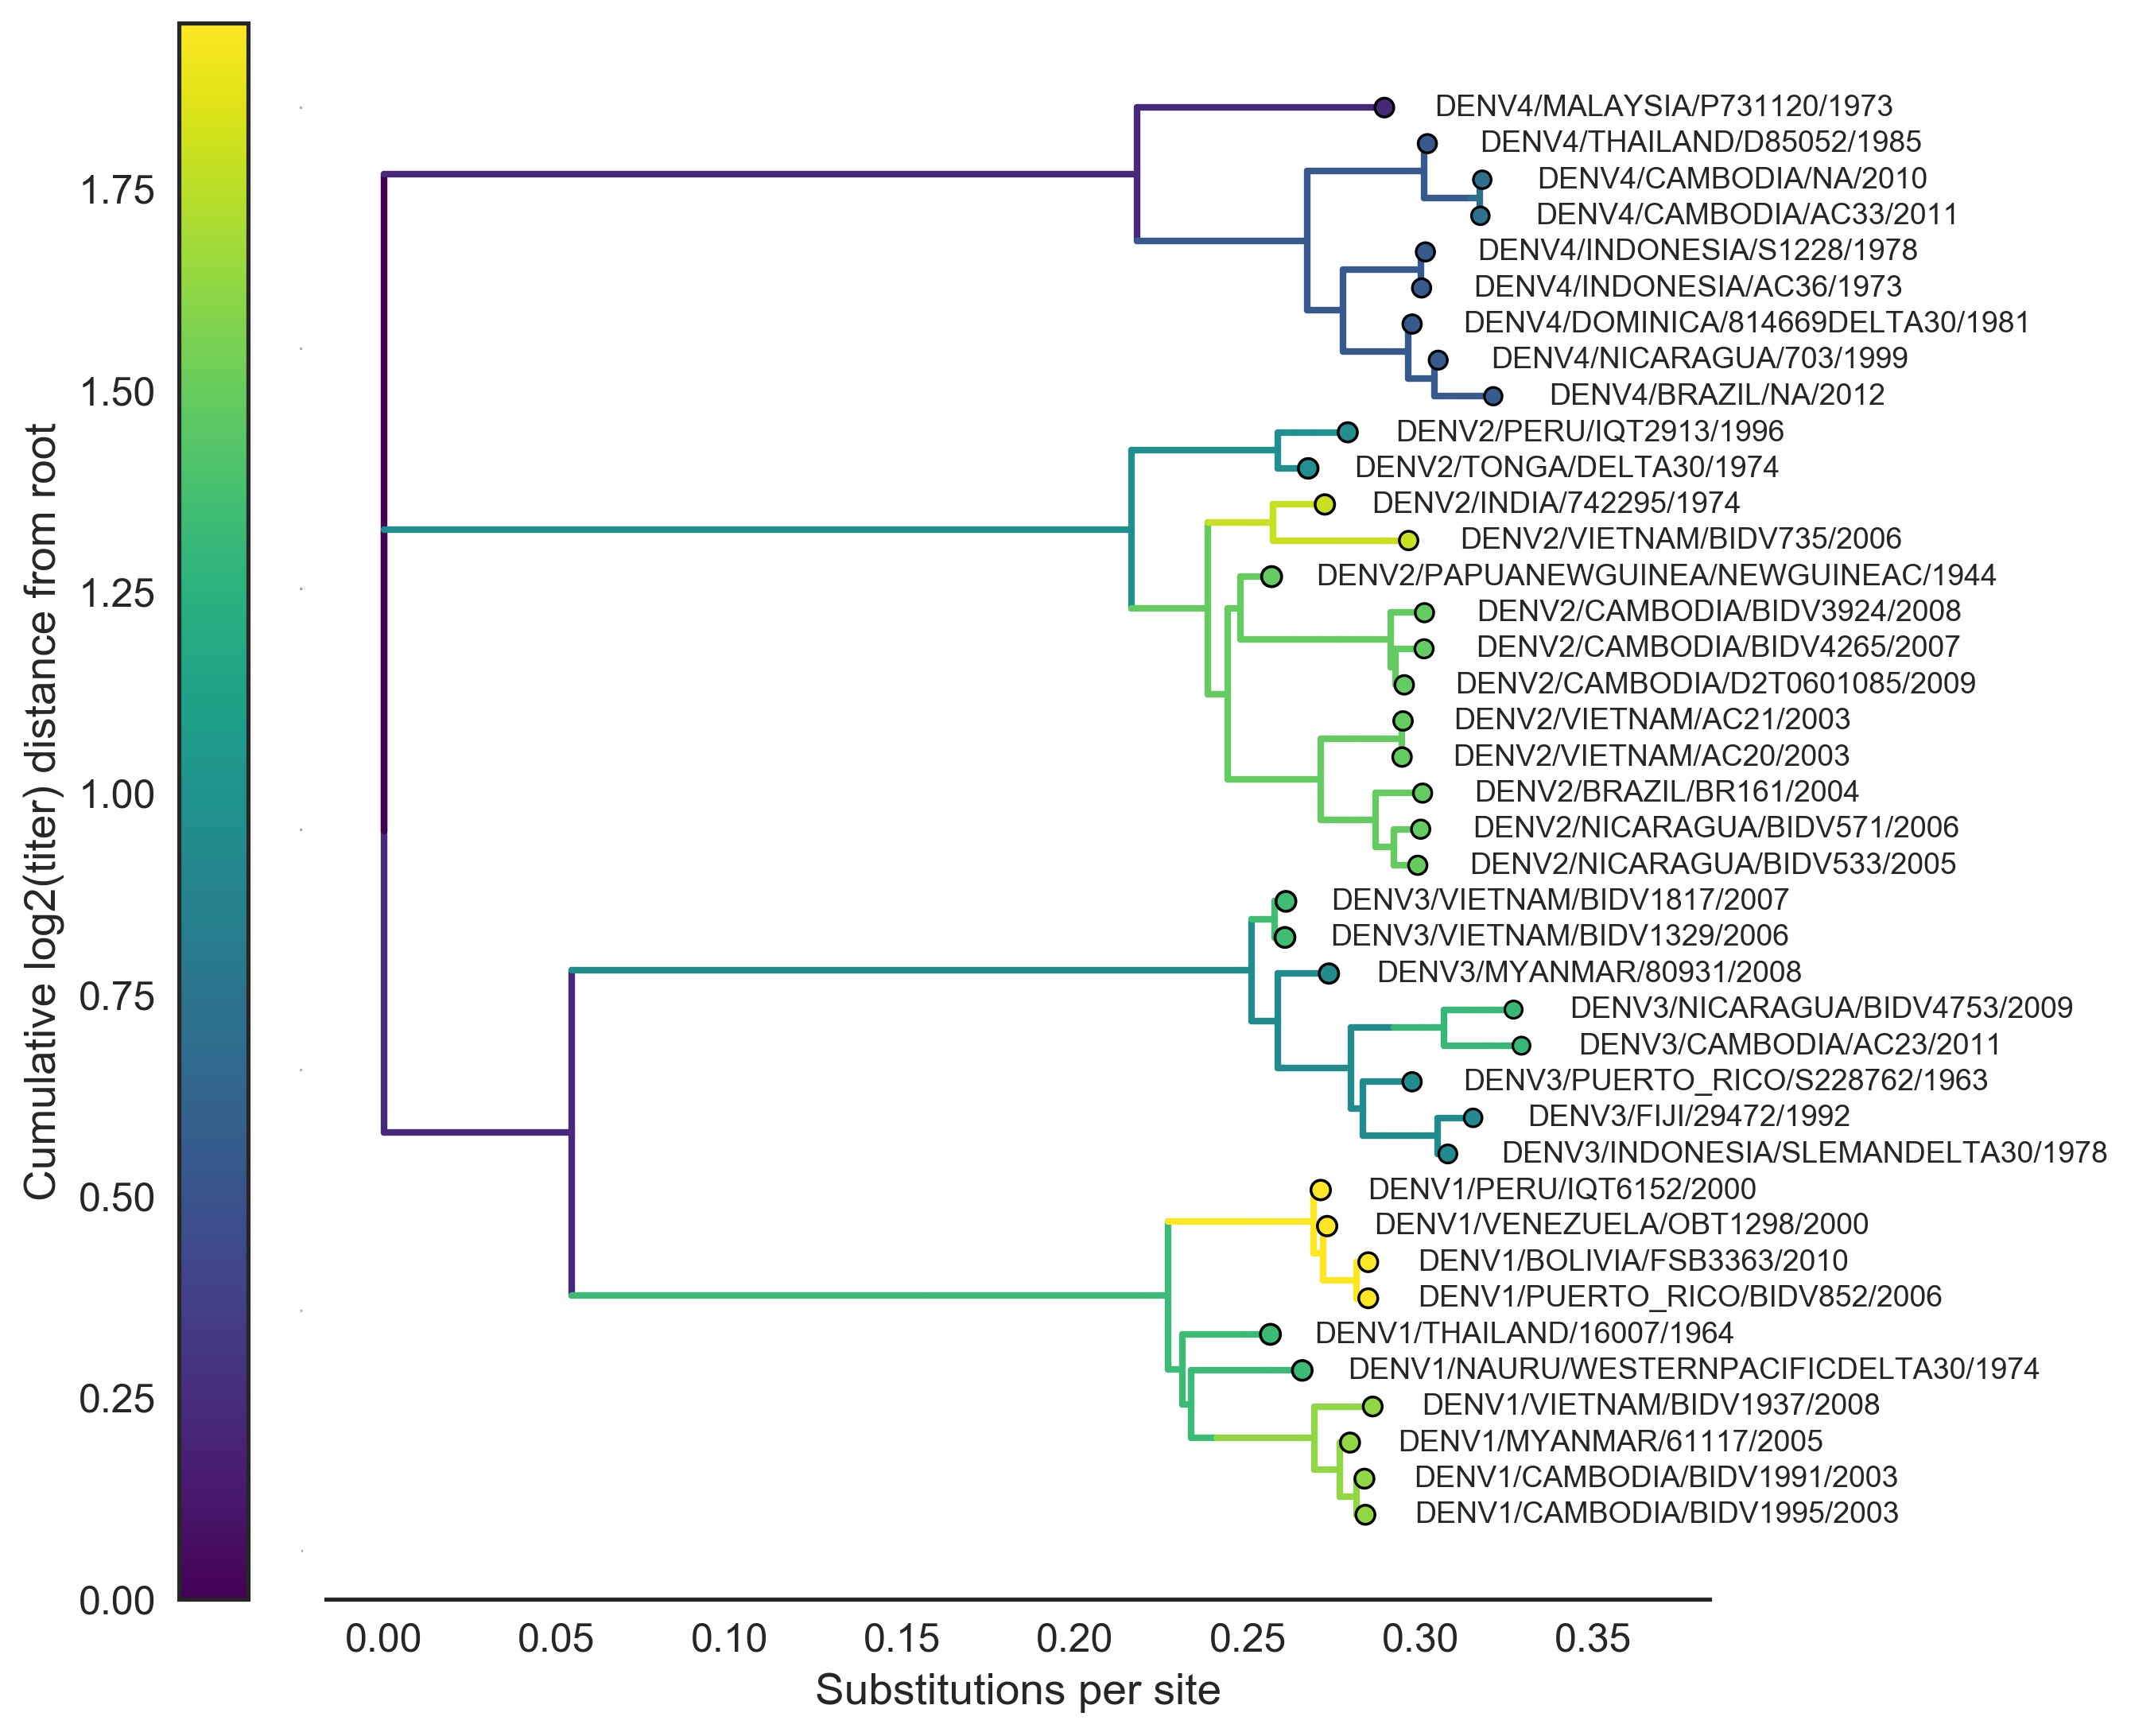
\includegraphics[width=0.75\textwidth]{../figures/png/titered_strains_tree.png}
	\caption{\textbf{Tree of DENV viruses in titer dataset}
  Maximum likelihood phylogeny of all DENV viruses that were included in the titer dataset.
	}
	\label{titered_strains_tree}
\end{figure}

\begin{figure}[h]
\centering
	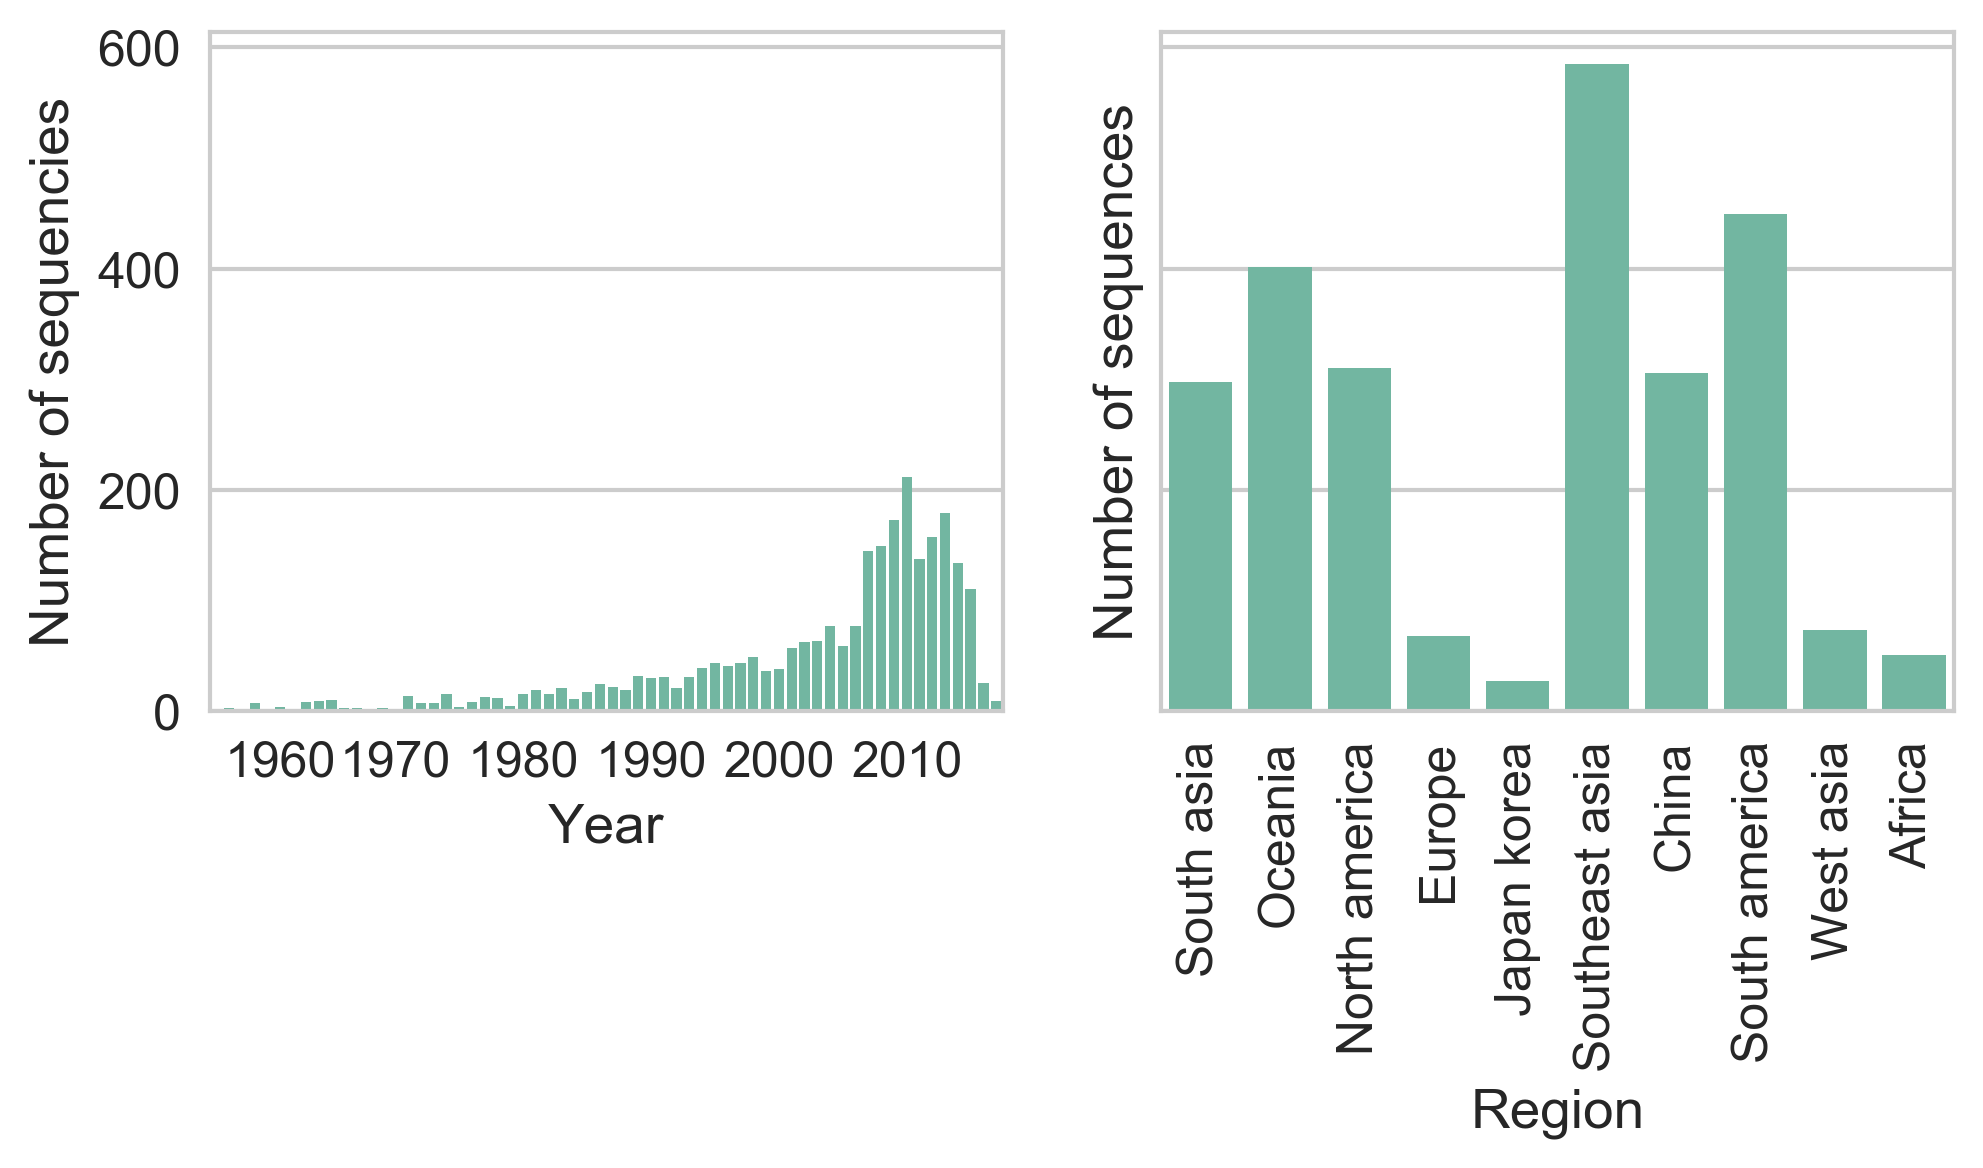
\includegraphics[width=0.75\textwidth]{../figures/png/sequence_distribution.png}
	\caption{\textbf{Sequence dataset distribution}
  Temporal and geographic distribution of sequences included in our dataset after subsampling.
	}
	\label{sequence_distribution}
\end{figure}

\begin{figure}[h]
  \centering
  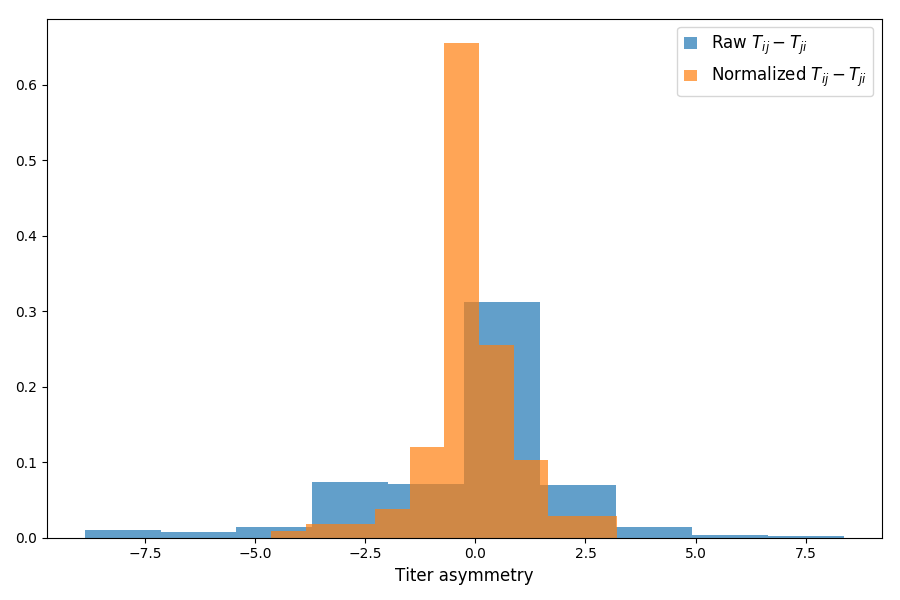
\includegraphics[width=0.5\textwidth]{../figures/png/titer_asymmetry.png}
  \caption{\textbf{Titer value symmetry}
  Some viruses have greater avidity overall, and some sera are more potent overall.
  We normalize for these row and column effects ($v_a$ and $p_b$, respectively) in the titer model.
  Once overall virus avidity and serum potency are accounted for, titers are roughly symmetric (i.e., $D_{ij} \approx D_{ji}$).
  }
\label{titer_asymmetry}
\end{figure}

\begin{figure}[h]
  \centering
  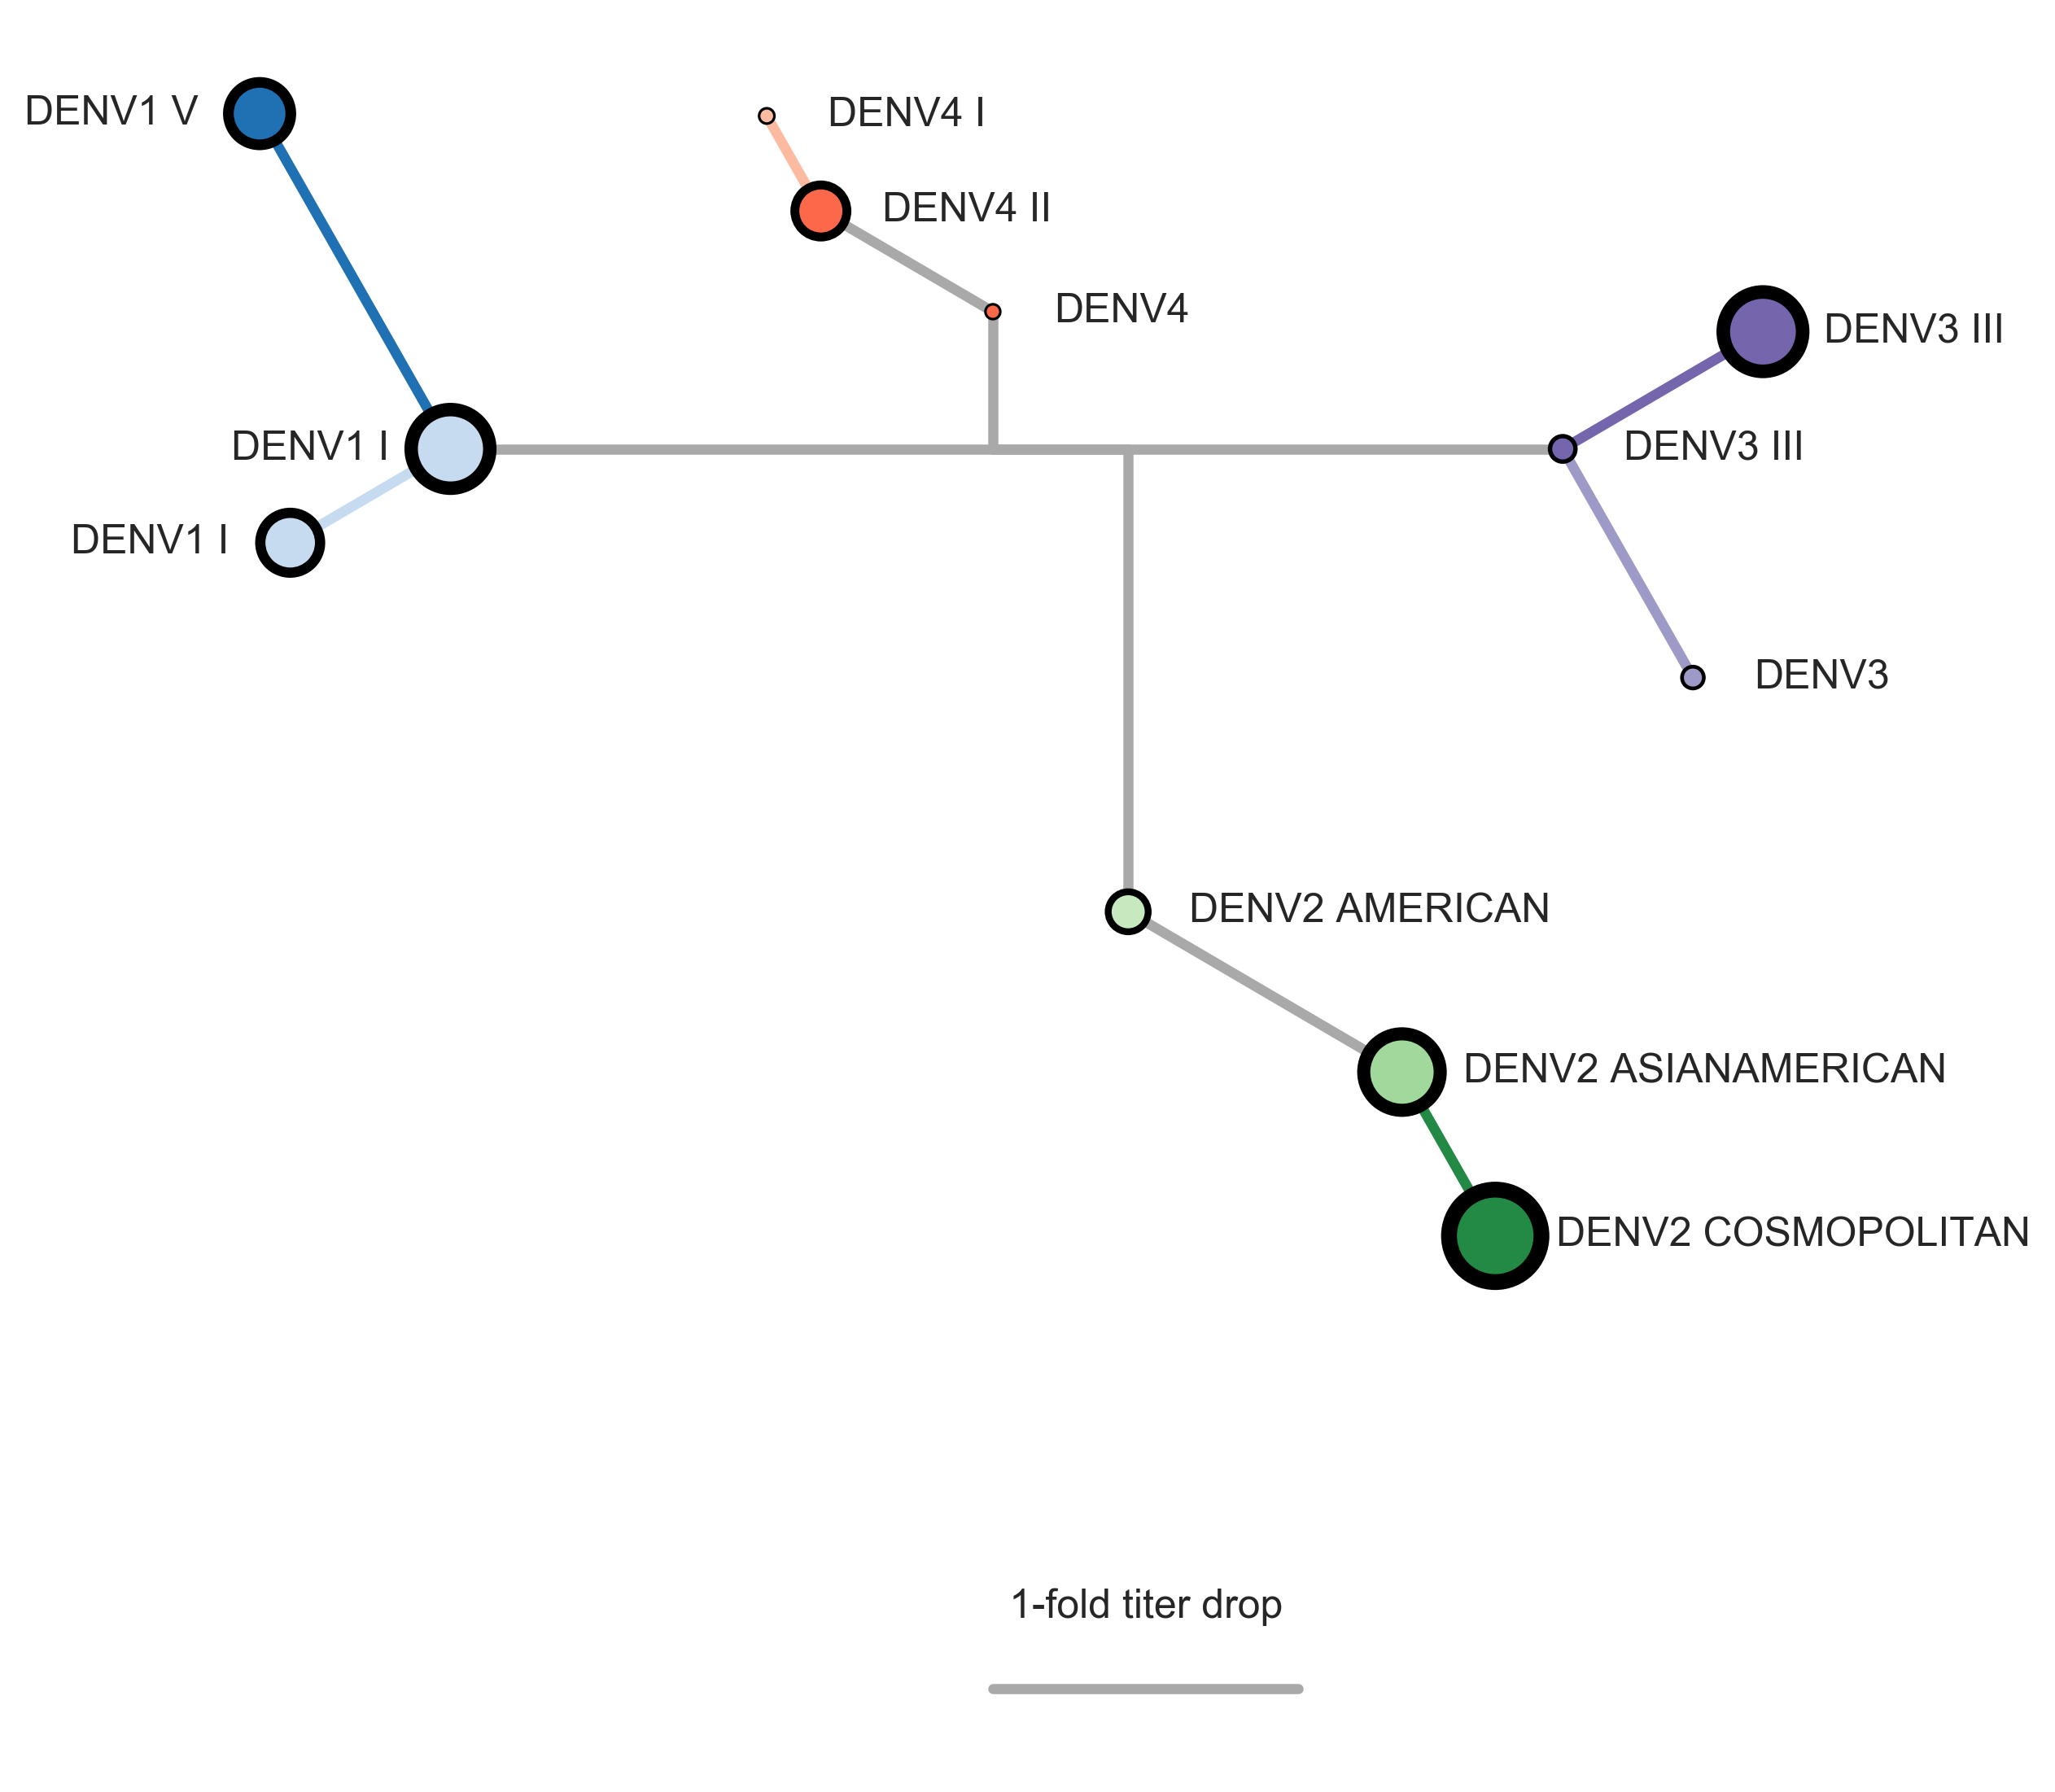
\includegraphics[width=\textwidth]{../figures/png/antigenic_tree_supplement.png}
  \caption{\textbf{Tree of dengue antigenic phenotypes (alternate view)}
As in Figure~\ref{antigenic_tree}, the topology is inferred from a maximum likelihood phylogeny of DENV sequences.
Branch lengths are scaled to represent the $d_b$ assigned to each branch by the `full tree' model of antigenic evolution.
  }
\label{antigenic_tree_supplement}
\end{figure}

\begin{figure}[h]
\centering
	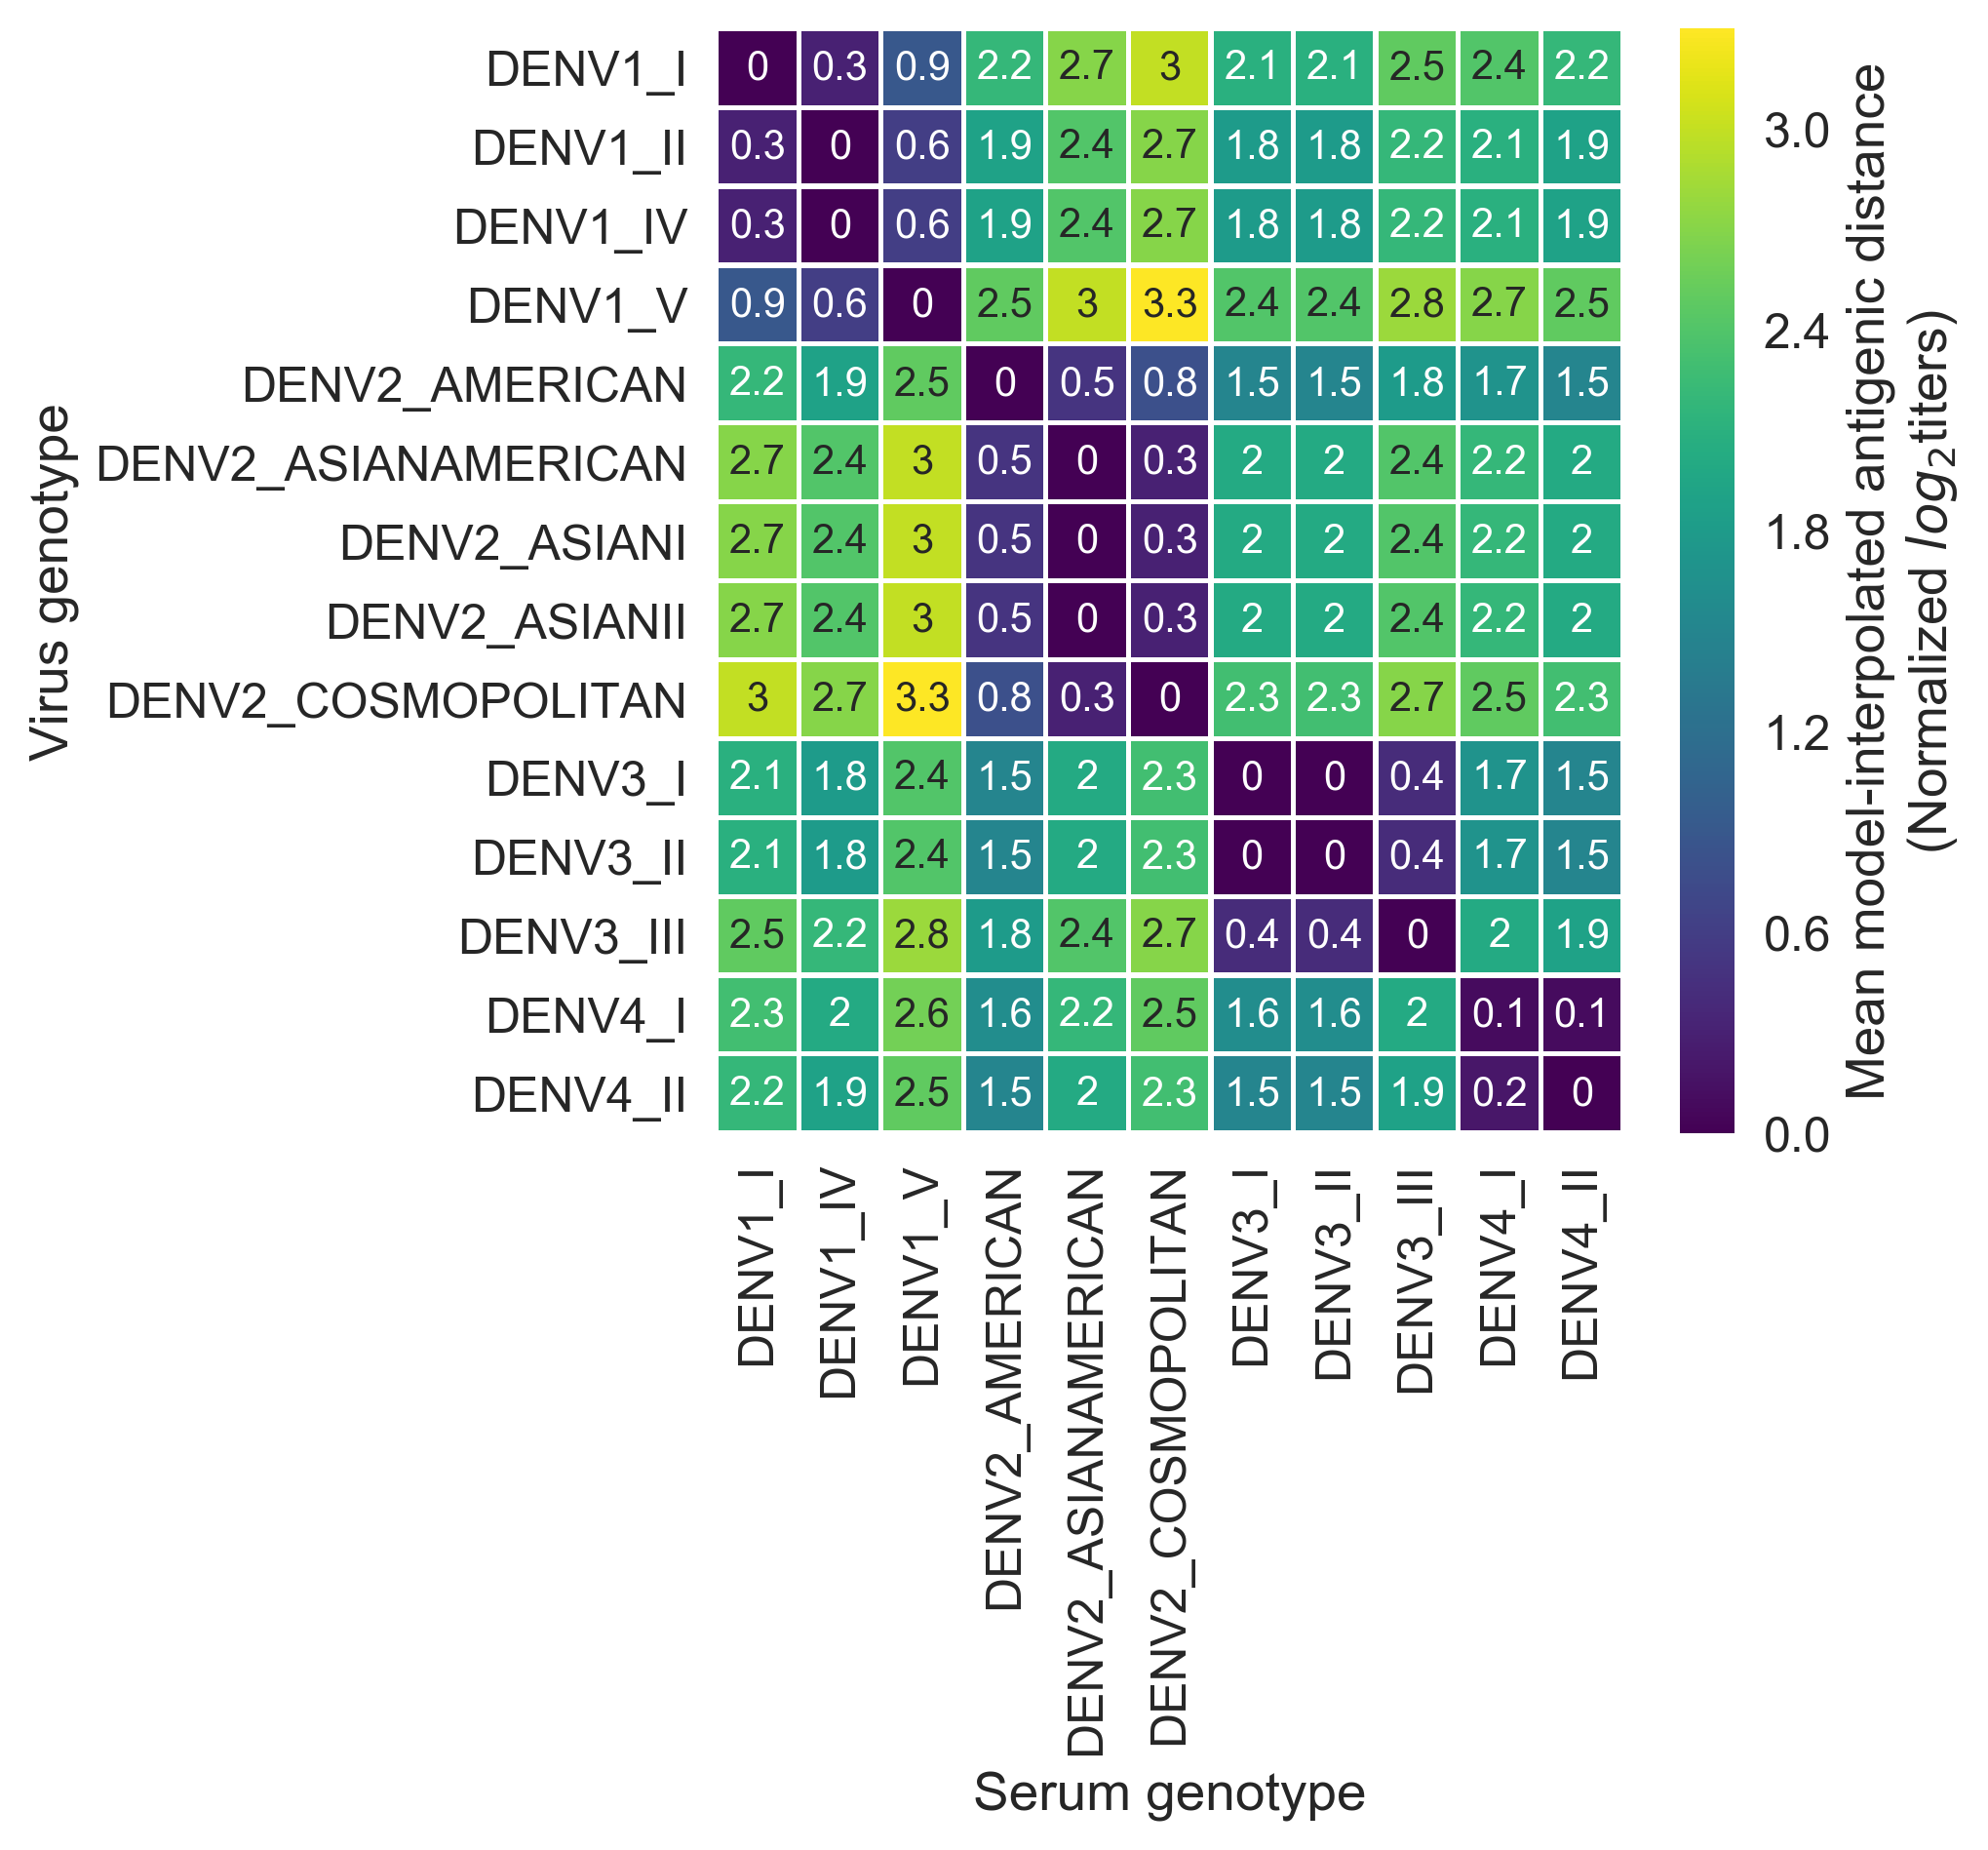
\includegraphics[width=0.75\textwidth]{../figures/png/genotype_dTiter_heatmap.png}
	\caption{\textbf{Titer distance by genotype}
  Values represent the mean interpolated antigenic distance between canonical dengue genotypes (in standardized log$_2$ titer units).
  }
	\label{genotype_dTiter_heatmap}
\end{figure}

% \renewcommand{\thetable}{S\arabic{table}}
%
% \begin{longtable}{ | r | l | p{2cm} | l | l | } % COLUMN FORMATS
%
%   \caption{TABLE CAPTION HERE} \label{TABLE LABEL HERE} \\
%   \endfirsthead
%
%   1 & KSA-378 & KJ713296 & camel & 2013-11 \\
%   2 & KSA-363 & KJ713298 & camel & 2013-11 \\
%   3 & KSA-503 & KJ713297 & camel & 2013-11 \\
%
% \end{longtable}

\end{document}
